\documentclass[conference]{IEEEtran}

\usepackage{amsmath,amssymb,amsfonts}
\usepackage{graphicx}
\usepackage{textcomp}
\usepackage{xcolor}
\usepackage{url}
\usepackage{array}
\usepackage{microtype}

\graphicspath{{images/}}

\begin{document}

\title{Secure AI-Powered Elderly Digital Safety Companion with Privacy-Preserving Scam Detection and Early Warning}

\author{
    \IEEEauthorblockN{
        Achinta R S\IEEEauthorrefmark{1},
        M Shreya\IEEEauthorrefmark{1},
        Dhanya\IEEEauthorrefmark{1},
        Kiranshree N\IEEEauthorrefmark{1}, and
        Fathima Mehnaz\IEEEauthorrefmark{2}
    }
    \IEEEauthorblockA{
        \IEEEauthorrefmark{1}Department of Computer Science and Engineering, \\
        Sahyadri College of Engineering \& Management, Mangaluru, Karnataka, India \\
        Email: \{achinta.cs21, shreya.cs21, dhanya.cs21, kiranshree.cs21\}@sahyadri.edu.in
    }
    \IEEEauthorblockA{
        \IEEEauthorrefmark{2}Project Guide, Department of Computer Science and Engineering, \\
        Sahyadri College of Engineering \& Management, Mangaluru, Karnataka, India \\
        Email: fathima.cs@sahyadri.edu.in
    }
}

\maketitle

\begin{abstract}
The rapid proliferation of digital communication and electronic payment ecosystems has exposed vulnerable demographics, particularly senior citizens, to increasingly sophisticated social engineering scams, smishing attacks, and credential-harvesting fraudulent URLs. Elderly individuals are disproportionately targeted due to reduced technical familiarity, cognitive vulnerabilities, and the psychological exploitation of fear, urgency, and authority impersonation. Existing anti-spam applications often rely on centralized contact-harvesting directories that violate user privacy, depend on sluggish reactive blacklists, transmit raw personal communications to third-party cloud servers, and present complex technical telemetry in foreign languages without actionable guidance. To address these critical limitations, this paper presents \textbf{SilverShield AI}, an intelligent, privacy-preserving digital safety companion engineered specifically for elderly users and their family caregivers. SilverShield AI features a decoupled microservice architecture integrating: (1) a lightweight machine learning scam detection engine powered by Term Frequency-Inverse Document Frequency (TF-IDF) feature extraction and a calibrated Logistic Regression classifier achieving 98.06\% accuracy, 93.75\% scam recall, and an ROC-AUC of 0.9963 across a curated corpus of 5,160 deduplicated messages; (2) a privacy-preserving 9-layer heuristic URL security inspection engine that operates entirely without outbound network requests, completely eliminating adversary telemetry; (3) a centralized multi-vector risk aggregation engine incorporating deterministic safety overrides (OVR-01--OVR-06); (4) OWASP Gold Standard Argon2id password hashing, timing-equalized authentication, and stateless JWT session management; and (5) a WCAG AAA compliant assistive interface providing tri-lingual localization in English, Hindi, and Kannada alongside browser-native multi-tier Web Speech narration. The entire platform enforces a strict zero-raw-message storage policy in compliance with DPDP and GDPR guidelines. Extensive automated verification across 162 unit, integration, and live service tests confirms that SilverShield AI provides robust, explainable, and accessible cyber protection for senior citizens.
\end{abstract}

\begin{IEEEkeywords}
Elderly Digital Safety, Scam Detection, Phishing URL Analysis, Privacy-Preserving AI, Explainable AI, Machine Learning, Assistive Technology, Cybersecurity.
\end{IEEEkeywords}

\section{Introduction}

\subsection{Background}
The global acceleration of digital transformation has migrated critical everyday services---including banking, utility payments, healthcare consultations, and pension distribution---onto mobile and web platforms. In emerging economies like India, the nationwide adoption of the Unified Payments Interface (UPI) and smartphone-based messaging platforms has brought millions of older adults online for the first time. While this digital connectivity offers unprecedented convenience and social inclusion, it has simultaneously created an expansive attack surface for cybercriminals. Senior citizens represent an exceptionally vulnerable segment in this digital ecosystem. Cyber fraudsters deploy sophisticated social engineering methodologies via Short Message Service (SMS), WhatsApp, and instant messaging, specifically engineered to exploit cognitive aging, lack of technical familiarity, and emotional triggers.

\subsection{Motivation}
Recent empirical criminological and cybersecurity studies reveal that cyber fraud targeting older adults is escalating in both frequency and financial severity. Scammers systematically utilize emotional manipulation techniques, including manufactured urgency (e.g., ``Account suspended within 2 hours''), fear-based intimidation (e.g., ``Electricity bill unpaid, power will be disconnected tonight''), lottery and reward deceptions, and impersonation of trusted institutions such as state banks (SBI, HDFC), regulatory authorities (RBI), tax departments, and law enforcement agencies. 

Despite the prevalence of these attacks, conventional cybersecurity solutions fail to protect elderly users due to five fundamental systemic shortcomings:
\begin{enumerate}
    \item \textbf{Privacy Invasions in Commercial Tools:} Mainstream commercial spam filters (e.g., Truecaller) operate by aggressively harvesting and centralizing users' entire address books and logging unencrypted communication metadata, creating severe privacy risks under modern data protection frameworks such as the European General Data Protection Regulation (GDPR) and India's Digital Personal Data Protection (DPDP) Act 2023.
    \item \textbf{Lagging Reactive Blacklists:} Traditional filters rely on crowdsourced phone number and domain blacklists. Consequently, they fail against zero-day smishing campaigns launched from freshly registered SIM cards and disposable, dynamically generated domains.
    \item \textbf{Adversary Telemetry from Active URL Crawling:} Many enterprise threat scanners actively fetch external links to inspect HTML payloads. This active network probing alerts malicious web servers that a target has clicked the link, verifying the active status of the victim's telephone number or IP address.
    \item \textbf{Cognitive and Linguistic Inaccessibility:} Existing security interfaces present cryptic technical jargon (e.g., ``SSL Certificate Common Name Mismatch'', ``DMARC Verification Failure'') in English-only formats with micro-typography, confusing senior citizens rather than empowering them.
    \item \textbf{Absence of Emergency Caregiver Escalation:} When an elderly user encounters an ambiguous message, current tools offer no automated, one-click bridge to consult trusted family caregivers or escalate to national cyber emergency helplines.
\end{enumerate}

\subsection{Objectives}
To mitigate these challenges, the primary objectives of the SilverShield AI project are:
\begin{enumerate}
    \item To design and implement a lightweight, high-performance content-based Natural Language Processing (NLP) and Machine Learning (ML) classifier capable of detecting smishing and financial scam messages with sub-5ms latency and an ultra-low False Negative Rate (FNR).
    \item To construct a 9-layer passive, privacy-preserving URL security analyzer that inspects lexical, architectural, and structural anomalies in hyperlinks without issuing outbound HTTP requests.
    \item To develop a centralized multi-vector risk engine that normalizes heterogeneous threat indicators into an objective risk score ($0$--$100$) governed by deterministic safety overrides.
    \item To establish an end-to-end privacy-by-design framework that enforces a zero-raw-message storage policy, memory-hard Argon2id authentication, anti-enumeration defenses, and granular consent management.
    \item To engineer an accessible, WCAG AAA compliant user interface providing tri-lingual support (English, Hindi, Kannada) and browser-native multi-tier speech synthesis for elderly users.
\end{enumerate}

\subsection{Contributions of the Proposed System}
The key academic and engineering contributions of this work include:
\begin{itemize}
    \item \textbf{Champion Scam Classifier with Minimal False Negatives:} We demonstrate that calibrated Logistic Regression with TF-IDF unigram and bigram features achieves a 93.75\% scam recall and 0.9963 ROC-AUC, outperforming Multinomial Naive Bayes by reducing false negatives by 50\% on benchmark SMS datasets.
    \item \textbf{Zero-Request Heuristic URL Inspection:} We introduce a 9-layer inspection pipeline (evaluating IP hosts, subdomain depth, URL shorteners, sensitive keywords, abusive TLDs, typosquatting via Levenshtein distance, unencrypted HTTP, string length, and Shannon entropy) that assesses link safety without leaving network footprints.
    \item \textbf{Explainable Safety Overrides:} Rather than outputting opaque probability values, the system translates mathematical predictions into 10 deterministic semantic intent indicators, clear plain-language warnings, and concrete actionable guidance tailored for non-technical seniors.
    \item \textbf{Multi-Tier Indic Speech Narration:} We implement an assistive speech narration subsystem that dynamically queries browser synthesis engines for native Indic voices (`kn-IN', `hi-IN'), providing audio assistance without garbling regional text.
    \item \textbf{Enterprise-Grade Security Architecture:} We incorporate memory-hard Argon2id password hashing ($m=64\text{ MiB}, t=2, p=1$), constant-time timing equalizers resisting username enumeration, sliding-window rate limiting, and stateless JWT token blacklisting.
\end{itemize}

\section{Literature Survey}

\subsection{Review of Main Research Papers}
To establish the theoretical and empirical foundation of SilverShield AI, we review four primary academic works spanning elderly scam vulnerability, modern phishing detection methodologies, privacy-preserving explainable architectures, and foundational SMS spam benchmark analysis.

\subsubsection{Elderly Imposter Scam Vulnerability}
In [1], L. R. Shapiro investigated the operational mechanisms and reporting patterns of cyber-enabled imposter scams targeting older adults in the United States. Published in the \textit{Security Journal} (2025), this study conducted an extensive empirical examination of reported fraud incidents, focusing on the sociodemographic, psychological, and technical vectors exploited by cybercriminals. Shapiro found that older adults are disproportionately victimized by imposter scams that simulate authority---such as government agencies, financial institutions, and tech support providers. Scammers rely on artificial urgency, threats of legal action, and emotional manipulation to bypass analytical decision-making. 

\textit{Contributions and Limitations:} The primary contribution of [1] is its rigorous criminological categorization of imposter scam narratives and its documentation of severe financial and psychological harm among seniors, alongside evidence of massive underreporting due to shame or cognitive decline. However, a major limitation of Shapiro's work is its exclusively retrospective and criminological scope; it does not propose, implement, or evaluate automated computational algorithms or real-time preventative cybersecurity tools. 

\textit{Relevance to SilverShield AI:} Shapiro's findings directly inform SilverShield AI's threat modeling. The 10 deterministic intent indicators engineered in our AI module---particularly authority impersonation, artificial urgency, threats of legal action, and bank KYC demands---are directly mapped to the exploitation vectors identified in [1]. Furthermore, Shapiro's observation regarding elderly isolation justifies our integration of one-click family caregiver alerting.

\subsubsection{Recent Advances in Phishing Detection}
In [2], S. Kavya and D. Sumathi presented a comprehensive review of emerging methodologies and state-of-the-art advances in phishing detection, published in \textit{Artificial Intelligence Review} (2025). The authors systematically examined machine learning, deep learning, heuristic, and hybrid detection frameworks across email, web, and URL vectors. They evaluated feature extraction strategies, including lexical URL properties, domain WHOIS metadata, visual page similarity, and NLP-driven message analysis.

\textit{Contributions and Limitations:} The study provides an exhaustive taxonomy of modern phishing countermeasures, comparing algorithmic trade-offs across classification accuracy, feature extraction latency, and resilience against adversarial evasion (such as typosquatting and URL obfuscation). Kavya and Sumathi emphasized that deep learning models (e.g., CNNs, LSTMs, Transformers) achieve high representation capability but incur substantial computational overhead, high inference latency, and severe black-box opacity. Conversely, traditional URL scanners depend heavily on real-time external network scraping, which introduces privacy vulnerabilities. 

\textit{Relevance to SilverShield AI:} This review establishes the rationale for SilverShield AI's architectural split. Rather than deploying heavy, opaque deep learning models or active web scrapers, we adopt lightweight, explainable linear classifiers paired with a 9-layer passive, zero-network-request URL heuristic engine, directly fulfilling Kavya and Sumathi's call for low-latency, interpretable defenses.

\subsubsection{Privacy-Preserving and Explainable Phishing Detection}
In [3], W. Li, Y. Liu, X. Chen, Z. Tan, and J. Ma proposed \textit{FedPhishLLM}, a privacy-preserving and explainable phishing detection mechanism combining federated learning and Large Language Models (LLMs), published in the \textit{Journal of King Saud University -- Computer and Information Sciences} (2025). Recognizing that centralized collection of user communications creates unacceptable privacy violations under GDPR, the authors developed a decentralized federated learning framework where client devices train local models and share only parameter gradients with a central aggregator. Furthermore, they fine-tuned an LLM to generate natural language explanations elucidating why a specific message was deemed malicious.

\textit{Contributions and Limitations:} The major contribution of [3] is the simultaneous formalization of cryptographic client privacy and transparent natural language explanation generation in phishing defense. However, FedPhishLLM suffers from significant practical constraints: running local LLMs and executing multi-round federated training rounds requires substantial local memory, powerful GPU acceleration, and heavy communication bandwidth. These hardware requirements make FedPhishLLM impractical for deployment on resource-constrained smartphones or commodity edge hardware used by senior citizens.

\textit{Relevance to SilverShield AI:} Li et al. strongly validate SilverShield AI's architectural mandate for privacy-by-design and explainable output. SilverShield AI achieves privacy preservation by enforcing a strict in-memory-only zero-raw-message storage rule on the local device, and delivers explainability via deterministic semantic indicators and plain-language action recommendations without requiring computationally prohibitive LLMs.

\subsubsection{Benchmark SMS Spam Filtering Study}
In [4], T. A. Almeida, J. M. G. Hidalgo, and A. Yamakami published their seminal work on mobile SMS spam filtering in the \textit{Proceedings of the 2011 ACM Symposium on Document Engineering (DocEng)}. The authors addressed the critical shortage of publicly available, non-synthetic SMS research datasets by creating the SMS Spam Collection corpus, consisting of 5,574 real-world English SMS messages tagged as legitimate (ham) or spam. They systematically trained and benchmarked standard machine learning classifiers, including Naive Bayes variants, Support Vector Machines (SVMs), and linear models, using diverse feature representation techniques.

\textit{Contributions and Limitations:} Almeida et al. established the definitive empirical benchmark for mobile SMS filtering that remains the gold standard in text cybersecurity research. They demonstrated that linear and probabilistic classifiers using TF-IDF feature extraction can achieve over 97\% classification accuracy on short, noisy mobile communications. However, the study has notable limitations: the dataset was collected in 2011 and lacks modern multi-stage smishing patterns, such as obfuscated shorteners, UPI banking fraud, and targeted spear-smishing. Additionally, the paper focused exclusively on binary classification metrics without addressing user-facing explainability, URL heuristic inspection, or elderly accessibility.

\textit{Relevance to SilverShield AI:} Almeida et al.'s corpus serves as the foundational training base for SilverShield AI's machine learning engine. In our system, this dataset is cleaned, rigorously deduplicated to 5,160 records, vectorized using advanced unigram and bigram TF-IDF representations, and integrated into a real-time production pipeline.

\begin{table*}[!t]
\centering
\caption{Comparative Analysis of Literature Survey Papers and Proposed SilverShield AI System}
\label{tab:literature_comparison}
\begin{tabular}{|p{2.2cm}|p{2.8cm}|p{3.2cm}|p{2.3cm}|p{2.8cm}|p{2.6cm}|}
\hline
\textbf{Research Work} & \textbf{Core Methodology} & \textbf{Key Contributions} & \textbf{Privacy Preservation} & \textbf{Explainability} & \textbf{Target Demographic} \\
\hline
\textbf{L. R. Shapiro (2025) [1]} & Empirical criminological survey of elderly scam incidents & Categorized authority fraud and psychological manipulation vectors & Theoretical review; no automated system & Descriptive post-incident statistics & Senior citizens (Victimology analysis) \\
\hline
\textbf{S. Kavya \& D. Sumathi (2025) [2]} & Systematic literature survey of ML/DL phishing detection & Evaluated trade-offs across feature sets, latency, and evasion & Evaluated external scrapers and databases & Surveyed model interpretability techniques & General Internet and enterprise users \\
\hline
\textbf{W. Li et al. (2025) [3]} & Federated learning coupled with Large Language Models & Decentralized model updates with natural language reasoning & High (Federated local training gradients) & High (LLM-generated natural language rationales) & General users with high-end hardware \\
\hline
\textbf{T. A. Almeida et al. (2011) [4]} & Bag-of-words / TF-IDF text classification on SMS data & Established definitive 5,574-message SMS Spam Collection corpus & Public static benchmark corpus & Binary classification score ($P(\text{spam})$) & General mobile telecommunication \\
\hline
\textbf{SilverShield AI (Proposed)} & Microservice NLP + 9-layer URL heuristics + Risk engine & Sub-5ms inference, zero-request URL audit, OVR-01--OVR-06 overrides & In-memory zero storage, Argon2id, DPDP/GDPR compliant & Deterministic intent tags + plain-language advice + audio & Senior citizens, non-tech users, caregivers \\
\hline
\end{tabular}
\end{table*}

\subsection{Comparative Analysis}
Table~\ref{tab:literature_comparison} provides a comprehensive comparative synthesis of the four analyzed research works alongside the proposed SilverShield AI architecture. As evidenced by the matrix:
\begin{itemize}
    \item Shapiro [1] provides vital behavioral insight into senior vulnerability but offers zero technological implementation.
    \item Kavya and Sumathi [2] comprehensively catalog algorithmic detection methodologies but highlight persistent trade-offs between deep learning latency, opacity, and privacy-invasive active crawling.
    \item Li et al. [3] provide an advanced privacy-preserving and explainable model via federated LLMs but incur prohibitive computational and hardware costs unsuitable for standard elderly client devices.
    \item Almeida et al. [4] provide the necessary empirical machine learning foundation for SMS filtering but lack modern smishing vectors, heuristic link analysis, explainability, and accessibility features.
\end{itemize}

\subsection{Identified Research Gap}
A synthesis of existing academic literature reveals four prominent, unresolved research gaps:
\begin{enumerate}
    \item \textbf{Disconnection Between Behavioral Gerontology and Engineering:} Existing cybersecurity tools are developed for enterprise or technically proficient users. The specific psychological manipulation tactics targeting older adults (authority impersonation, medical panic, utility disconnection) are rarely translated into real-time computational detection heuristics.
    \item \textbf{The Efficiency--Privacy Dilemma in URL Analysis:} Existing URL scanners either perform active HTTP requests that alert threat infrastructure and leak client IP telemetry, or query remote centralized blacklists that log user browsing history. There is a lack of lightweight, completely offline, zero-network-request heuristic URL inspection models.
    \item \textbf{The Inaccessibility of Explainable AI (XAI):} Existing explainable AI frameworks either generate complex mathematical feature attributions (SHAP/LIME values) incomprehensible to seniors, or require resource-heavy LLMs that cannot execute on commodity client hardware.
    \item \textbf{Absence of Multilingual Assistive Delivery:} Mainstream protective software completely overlooks non-English native speakers in developing nations, lacking regional localization and resilient, browser-native speech synthesis.
\end{enumerate}

\subsection{How SilverShield AI Addresses the Identified Gaps}
SilverShield AI directly bridges these gaps through an integrated sociotechnical architecture:
\begin{itemize}
    \item It operationalizes the psychological threat vectors identified by Shapiro [1] into 10 deterministic semantic intent rules and automated caregiver escalation channels.
    \item It implements a 9-layer passive URL heuristic engine that operates entirely in memory without issuing outbound network requests, completely avoiding adversary telemetry and external blacklist tracking.
    \item It delivers explainability without heavy LLMs by translating calibrated ML probabilities and heuristic flags into plain-language warnings and concrete action checklists.
    \item It solves linguistic and cognitive barriers through WCAG AAA accessible design, full tri-lingual localization (English, Hindi, Kannada), and a resilient multi-tier Web Speech narration engine tailored for Indic languages.

\end{itemize}

\section{Problem Formulation}

\subsection{Problem Definition}
Let an incoming communication received by an elderly user be defined as an event $E = (M, U, C, t)$, where $M \in \mathcal{S}^*$ represents the textual message string, $U = \{u_1, u_2, \dots, u_k\}$ denotes the set of hyperlinks embedded within $M$, $C$ represents the user's localized language context ($C \in \{\text{English}, \text{Hindi}, \text{Kannada}\}$), and $t$ is the event timestamp. 

The objective of SilverShield AI is to compute a deterministic risk assessment function $\Phi(M, U) \to (R, S, \mathcal{I}, \mathcal{W}, \mathcal{A})$, where:
\begin{itemize}
    \item $R \in \{\text{SAFE}, \text{LOW}, \text{MEDIUM}, \text{HIGH}\}$ is the categorical risk rating.
    \item $S \in [0.0, 1.0]$ is the normalized continuous threat score.
    \item $\mathcal{I} = \{i_1, i_2, \dots, i_m\}$ is the set of human-interpretable threat indicators.
    \item $\mathcal{W}$ is a localized plain-language warning message.
    \item $\mathcal{A} = \{a_1, a_2, \dots, a_n\}$ is an actionable safety advisory.
\end{itemize}
This computation must strictly satisfy:
\begin{equation}
    \text{Latency}(\Phi) < 50\text{ ms}, \quad \text{DiskIO}(M, U) = 0, \quad \text{OutboundNet}(U) = 0
\end{equation}
ensuring real-time execution, zero raw message storage, and zero outbound network probing.

\subsection{Existing Systems}
Existing protective systems fall into three primary categories:
\begin{enumerate}
    \item \textbf{Caller ID and Spam Blockers (e.g., Truecaller):} Rely on crowdsourced telephone number databases and user community tagging.
    \item \textbf{Commercial Safe Browsing Engines (e.g., Google Safe Browsing):} Rely on centralized URL blacklists generated via automated web crawlers and hash-prefix lookups.
    \item \textbf{Mobile Operating System Filters:} Native iOS and Android spam filters utilizing on-device heuristics or cloud synchronization.
\end{enumerate}

\subsection{Limitations of Existing Systems}
\begin{itemize}
    \item \textbf{Vulnerability to Zero-Day Campaigns:} Number blacklists are rendered useless when scammers purchase fresh virtual VoIP numbers or pre-activated SIM cards.
    \item \textbf{Intrusive Contact Harvesting:} Commercial caller ID platforms require full contact book upload, compromising the privacy of non-consenting third parties.
    \item \textbf{Attacker Notification via Web Crawlers:} Active scanning tools send HTTP GET requests to target URLs, signaling to cybercriminals that an attack vector is active.
    \item \textbf{Cognitive Friction:} Warnings such as ``Deceptive site ahead -- net::ERR\_CERT\_AUTHORITY\_INVALID'' induce confusion and anxiety in older users.
    \item \textbf{Monolingual Silos:} Lack of regional language synthesis isolates millions of non-English literate seniors.
\end{itemize}

\subsection{Proposed System}
SilverShield AI provides an integrated, 4-tier microservice architecture that decouples frontend presentation from backend analytical services. Incoming text and URLs are processed simultaneously by an AI/ML Scam Detection Engine (Member 2) and a 9-Layer URL Security Engine (Member 3). A Central Risk Aggregator (Member 4) synthesizes the threat signals into an explainable, normalized score governed by deterministic safety overrides, which is rendered on a WCAG AAA compliant assistive interface (Member 1) supporting English, Hindi, and Kannada speech narration.

\subsection{Advantages of Proposed System}
\begin{itemize}
    \item \textbf{Zero Raw Message Storage:} Raw communications and URLs are processed strictly in volatile memory (RAM) and immediately discarded.
    \item \textbf{Zero Outbound Telemetry:} URL heuristic analysis does not connect to the remote host, guaranteeing complete adversary blind spots.
    \item \textbf{Minimal False Negatives:} The calibrated Logistic Regression classifier achieves 93.75\% scam recall, minimizing the dangerous risk of missing an active scam.
    \item \textbf{Elderly Accessibility:} Large tap targets ($\ge 44\text{px}$), dynamic font scaling, high-contrast palette, and multi-tier browser-native speech synthesis.
    \item \textbf{Caregiver Support:} Direct one-click WhatsApp alert dispatching and integrated speed-dialing to India's National Cyber Crime Helpline `1930'.
\end{itemize}

\section{Project Design and Implementation}

\subsection{Overall System Architecture}
The system architecture of SilverShield AI follows a decoupled, service-oriented topology across four independent local microservices, as depicted in Fig.~\ref{fig:system_architecture}.
\begin{itemize}
    \item \textbf{Tier 1: Assistive Frontend (Port 8501):} Implemented in Python using Streamlit, featuring custom CSS styling, dynamic accessibility modes, and HTML5 Web Speech audio narration embedding.
    \item \textbf{Tier 2: Central Risk Integration API (Port 8000):} Developed using FastAPI, serving as the core orchestrator managing authentication, database persistence, consent audit logs, and risk synthesis.
    \item \textbf{Tier 3: AI/ML Scam Detection API (Port 8001):} Dedicated FastAPI service executing TF-IDF feature extraction, Logistic Regression inference, and intent indicator pattern matching.
    \item \textbf{Tier 4: URL Security API (Port 8002):} Dedicated FastAPI service executing 9-layer zero-request heuristic URL inspection and URL sanitization.
\end{itemize}

\begin{figure}[!t]
\centering
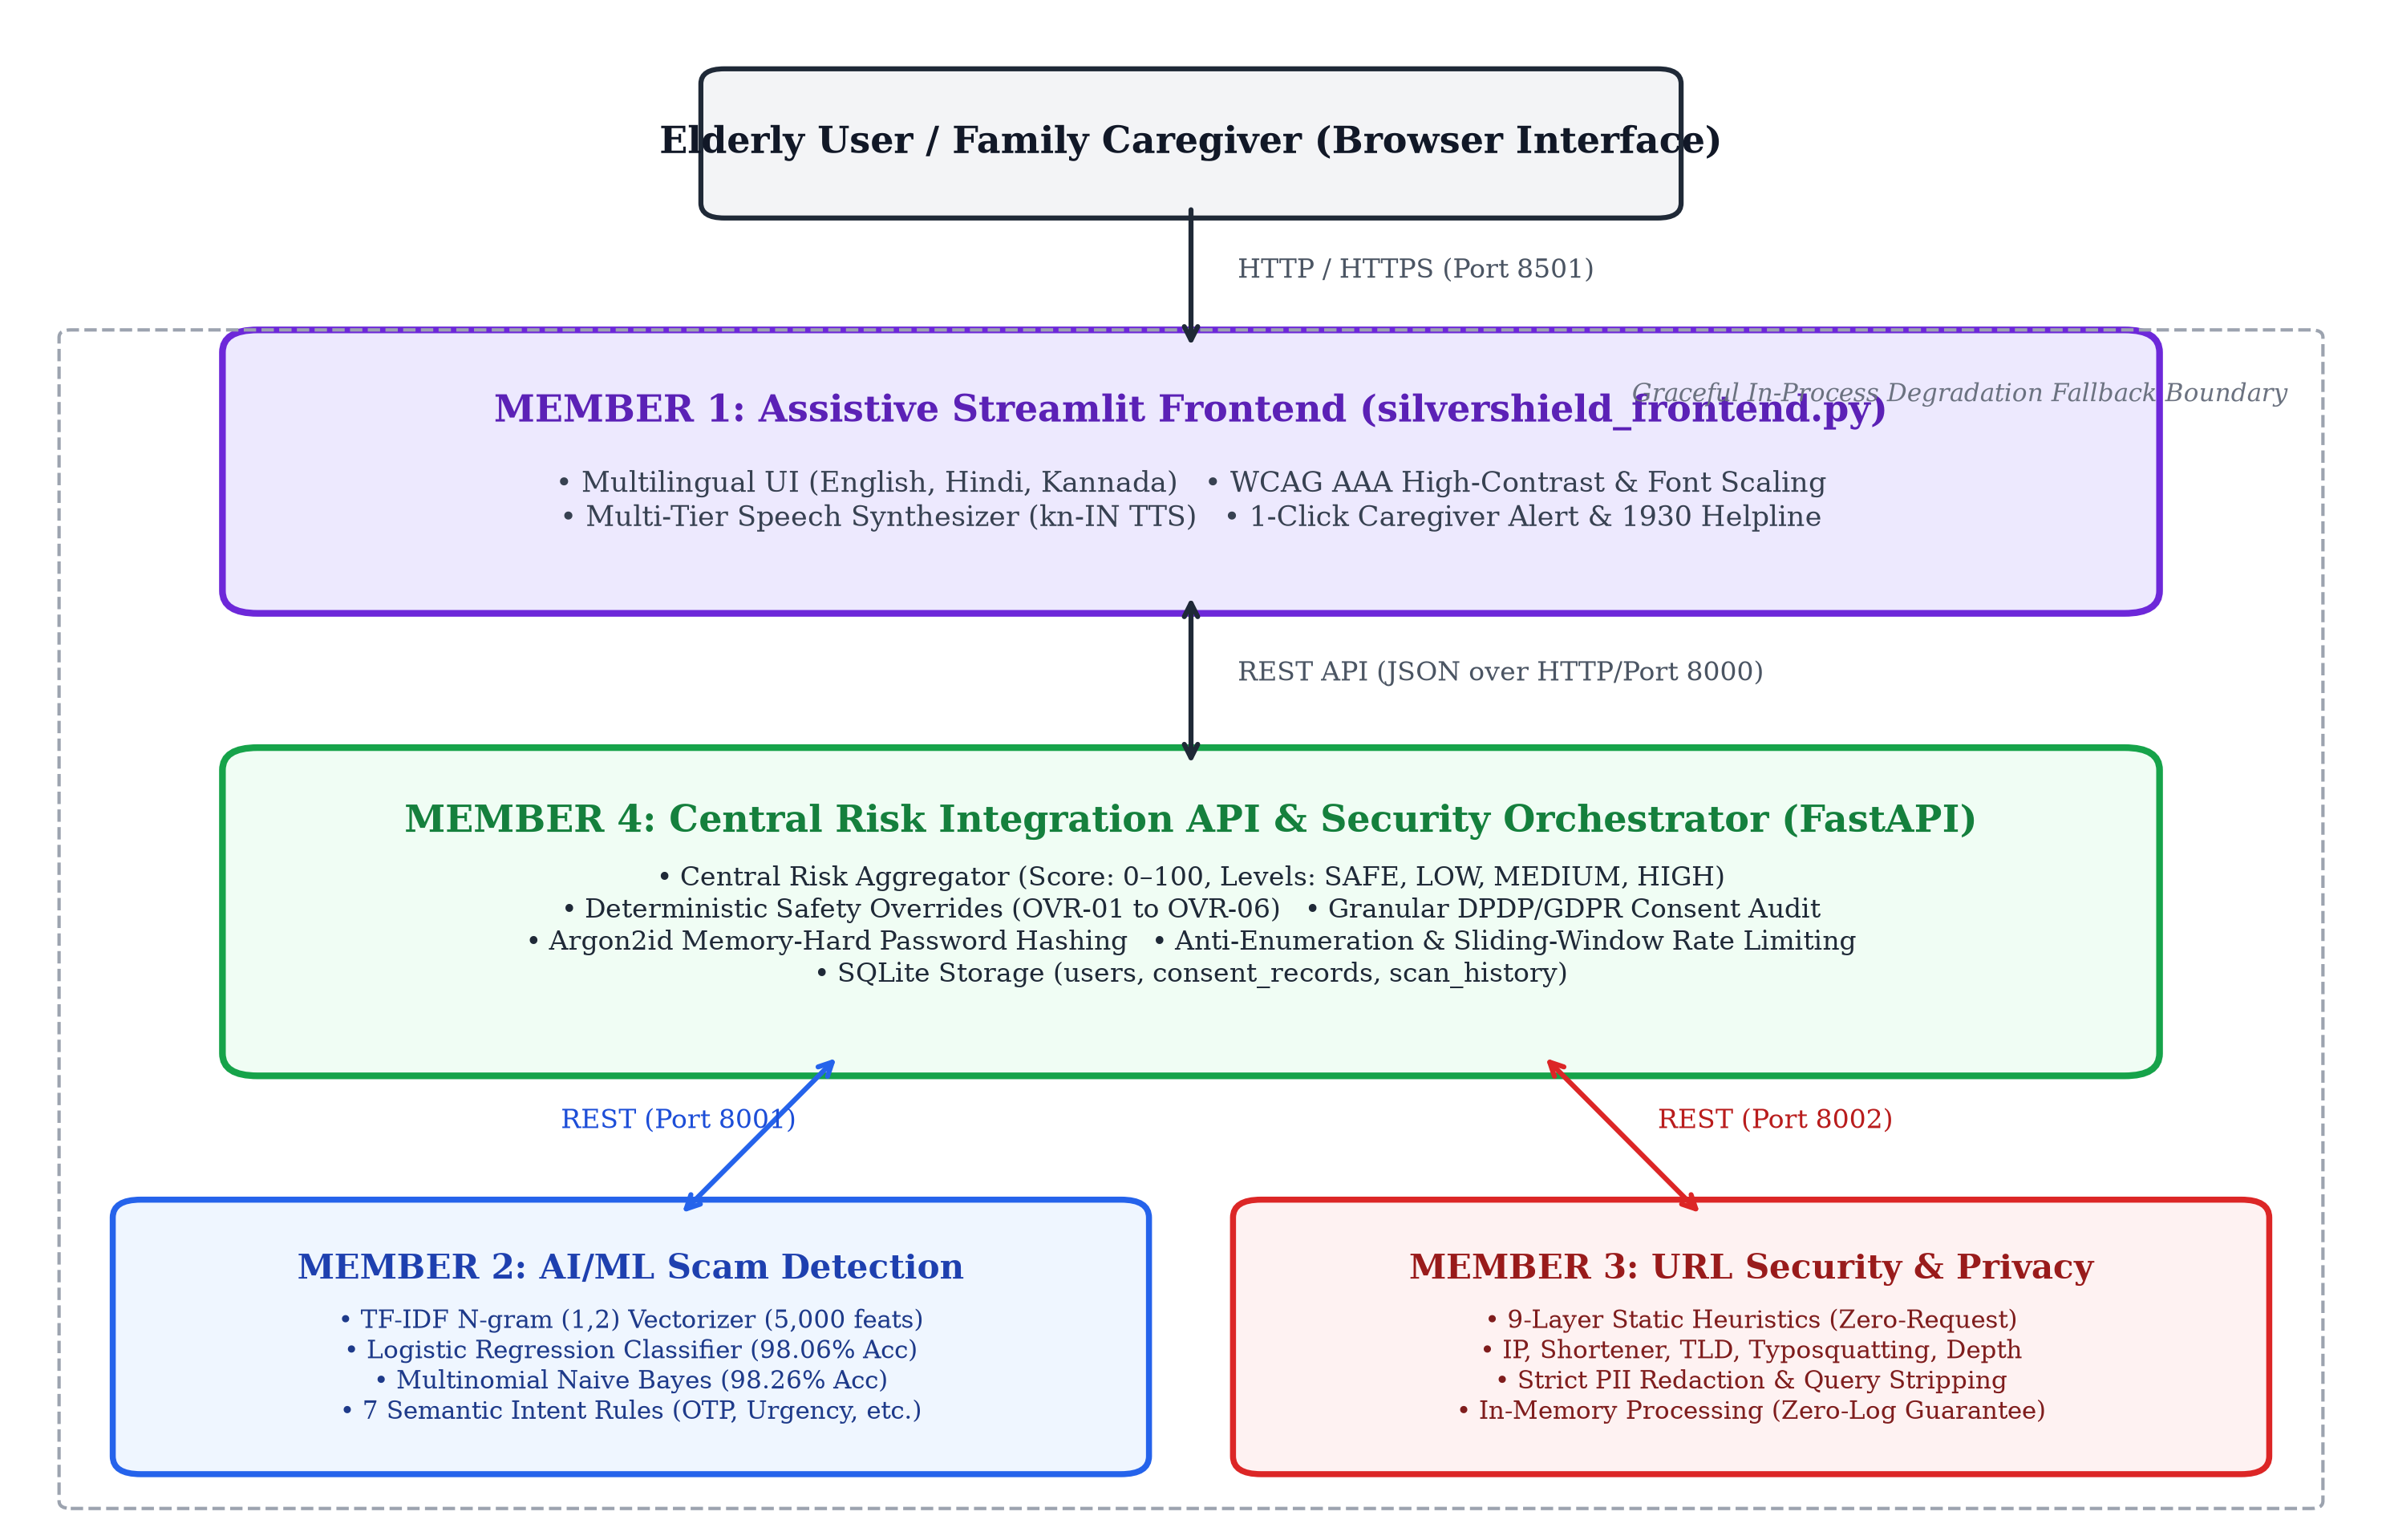
\includegraphics[width=\columnwidth]{fig1_system_architecture.png}
\caption{SilverShield AI 4-Tier Microservice System Architecture illustrating communication flows across ports 8501, 8000, 8001, and 8002, alongside persistent SQLite storage and the graceful in-process degradation fallback.}
\label{fig:system_architecture}
\end{figure}

\begin{figure}[!t]
\centering
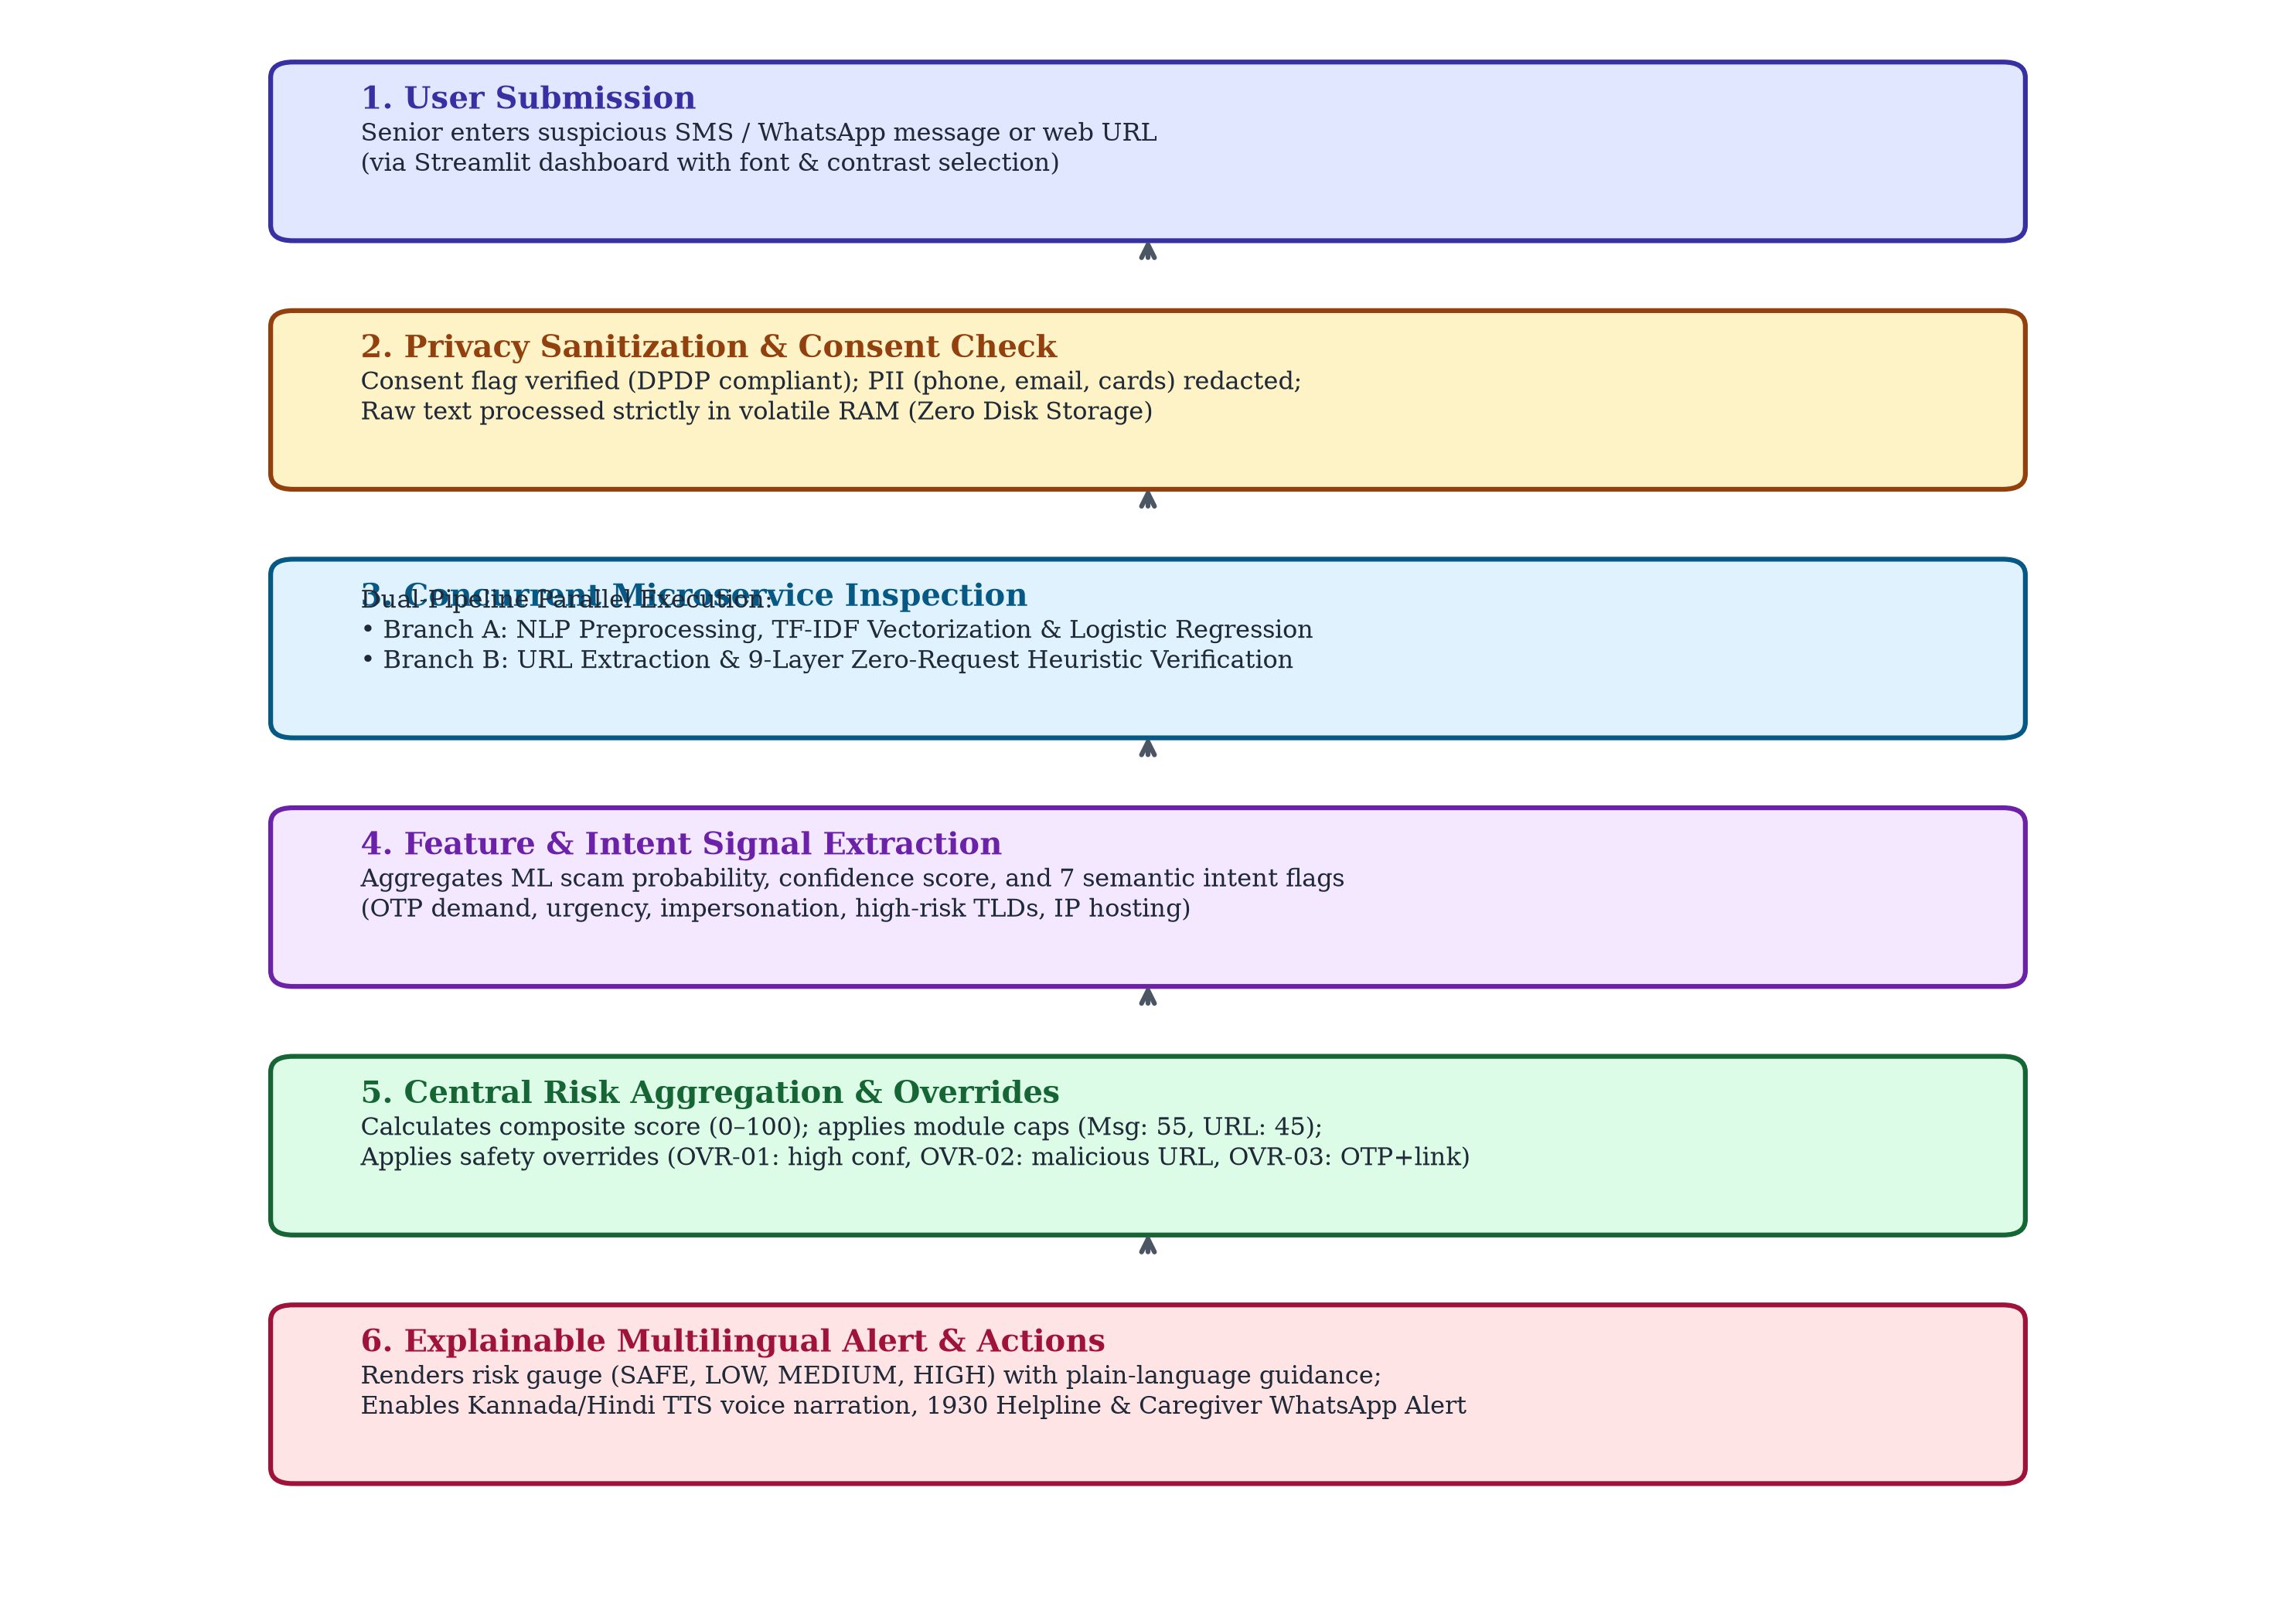
\includegraphics[width=\columnwidth]{fig2_system_workflow.png}
\caption{End-to-End System Workflow diagram depicting user submission, asynchronous microservice dispatch, risk score calculation, safety override evaluation, and multimodal advisory generation.}
\label{fig:system_workflow}
\end{figure}

\subsection{Graceful In-Process Degradation}
To ensure continuous availability, SilverShield AI implements automatic graceful degradation. If any microservice becomes unreachable over its network port:
\begin{itemize}
    \item If the ML Scam API (Port 8001) is down, the orchestrator sets status to `DEGRADED', logs `state=UNAVAILABLE', and activates a minimum safety floor so suspicious inputs are never erroneously marked safe.
    \item If the URL Security API (Port 8002) is down, text scam analysis proceeds normally while URL status reports `UNAVAILABLE'.
    \item If the Central Integration API (Port 8000) is unreachable when the Streamlit frontend boots, Streamlit seamlessly switches to its built-in \textbf{Local AI Security Engine}, executing the ML models and URL heuristics directly in-process with identical classification accuracy.
\end{itemize}

\subsection{System Workflow}
The runtime execution sequence is illustrated in Fig.~\ref{fig:system_workflow}. Upon user submission of a message or URL:
\begin{enumerate}
    \item The client verifies consent and sanitizes the input string.
    \item The Central API parses the payload, extracts any embedded hyperlinks, and issues concurrent REST calls to Ports 8001 and 8002.
    \item Port 8001 computes the scam probability and checks for 10 deterministic intent indicators.
    \item Port 8002 applies 9 heuristic inspection layers to the URL structure without making network contact.
    \item Port 8000 aggregates the individual threat vectors, applies source caps and safety overrides (OVR-01--OVR-06), and normalizes the score to $[0, 100]$.
    \item The final response is delivered to the frontend, which renders localized text warnings and initiates multi-tier audio synthesis.
\end{enumerate}

\subsection{Frontend Implementation}
The user interface (`silvershield_frontend.py`) is engineered to conform strictly to WCAG AAA accessibility standards:
\begin{itemize}
    \item \textbf{Color Palette:} Built on an accessible Deep Purple (`\#49316F`), Primary Purple (`\#7653B5`), Soft Lavender (`\#EDE5FA`), and Pure White (`\#FFFFFF`) design system (`frontend/styles.py`), achieving contrast ratios exceeding $7:1$.
    \item \textbf{High-Contrast Dark Mode:} A one-click toggle switches the interface to an ultra-high-contrast palette (`\#0B0814` background, `\#FFFFFF` text, `\#B39DDB` borders).
    \item \textbf{Dynamic Font Scaling:} Three distinct typographic scales: Compact (14px), Standard (15px), and Large (17px).
    \item \textbf{Touch Ergonomics:} All interactive buttons and cards maintain a minimum touch target size of $44 \times 44\text{ pixels}$.
\end{itemize}

\subsection{Backend Implementation}
The backend (`app/main.py`) is constructed using FastAPI and Pydantic v2 schemas. It exposes strict REST endpoints for `/api/v1/analyze`, `/api/v1/auth`, `/api/v1/consent`, and `/api/v1/health`. All endpoints feature automated input validation, structured error responses, and CORS security controls.

\begin{figure}[!t]
\centering
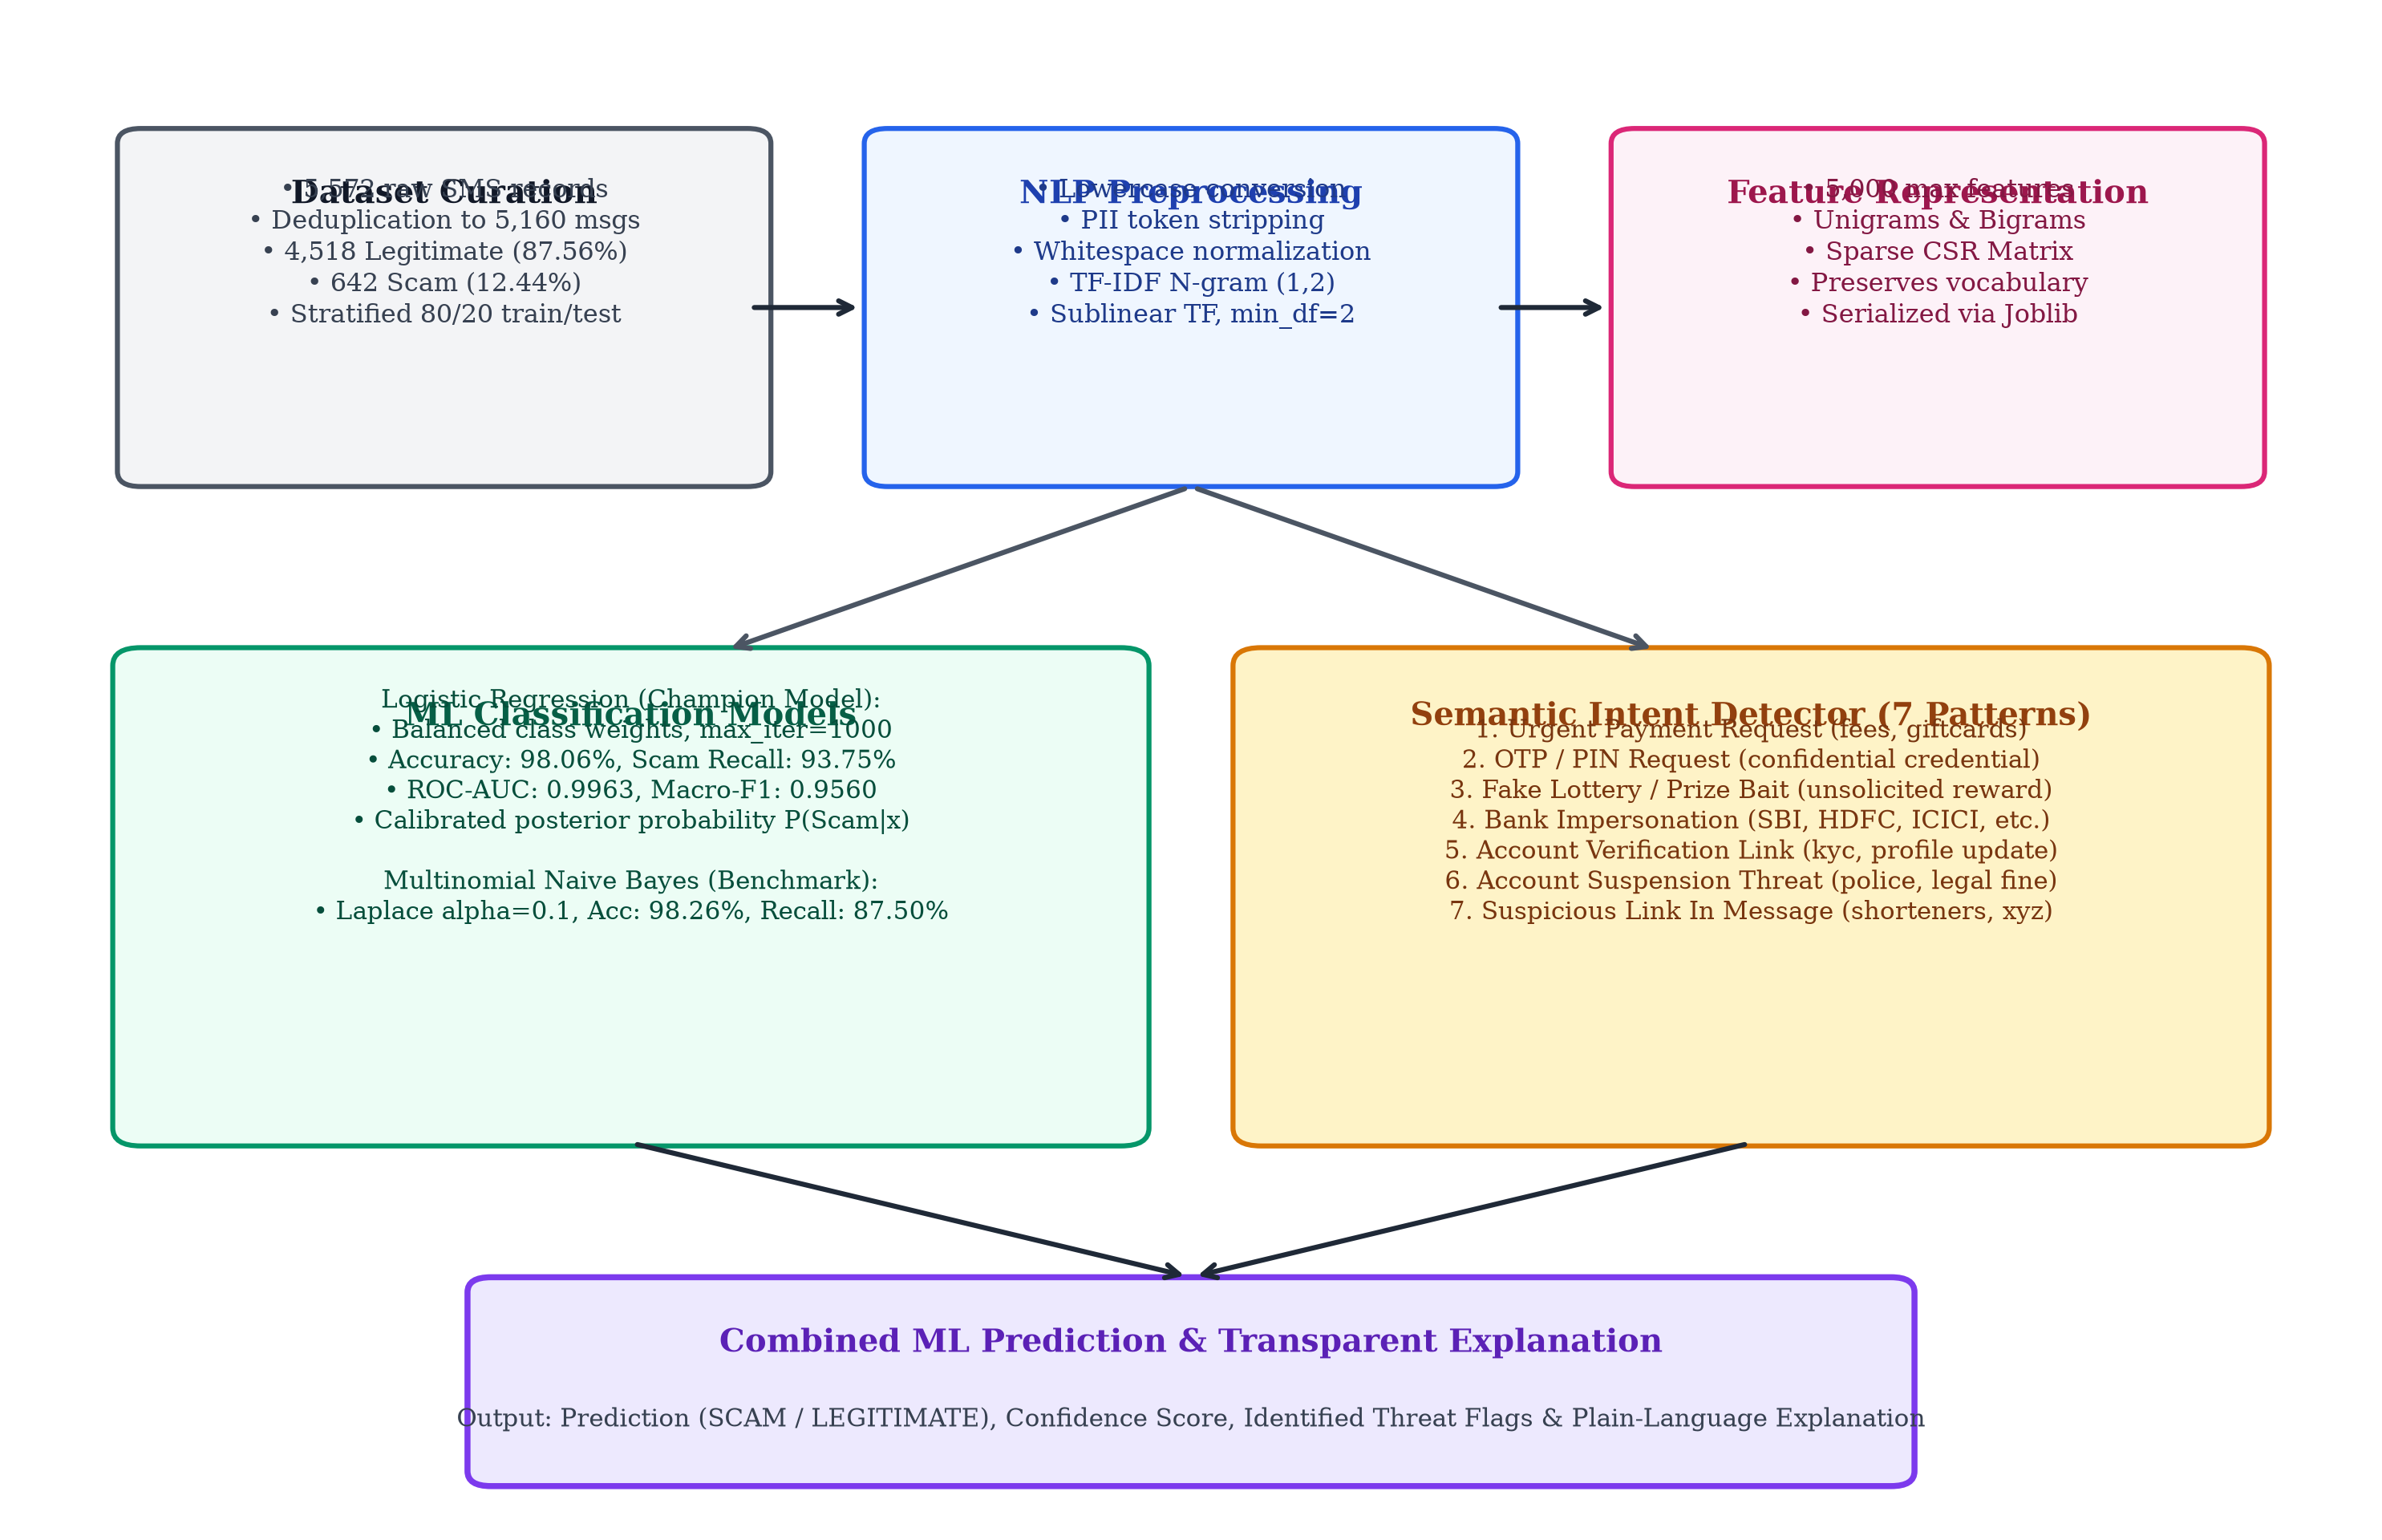
\includegraphics[width=\columnwidth]{fig3_ml_workflow.png}
\caption{AI/ML Scam Detection Pipeline illustrating text normalization, TF-IDF n-gram vectorization, Logistic Regression classification, and deterministic intent indicator matching.}
\label{fig:ml_workflow}
\end{figure}

\subsection{AI/ML Scam Detection Pipeline}
The machine learning pipeline (`ai_module/src/`), depicted in Fig.~\ref{fig:ml_workflow}, comprises dataset curation, textual preprocessing, feature extraction, and model inference.

\subsubsection{Dataset Description}
The model was trained on a verified SMS corpus (`ai_module/dataset/sms_scam_dataset.csv`). As detailed in Table~\ref{tab:dataset_stats}, the initial raw collection contained 5,572 records. We conducted rigorous automated deduplication, identifying and removing 412 duplicate messages (7.39\%), resulting in a clean corpus of 5,160 records comprising 4,518 legitimate messages (87.56\%) and 642 scam messages (12.44\%). The dataset was partitioned using an 80/20 stratified split into 4,128 training records and 1,032 independent testing records, preserving class distributions.

\begin{table}[!t]
\centering
\caption{Dataset Distribution and Split Statistics}
\label{tab:dataset_stats}
\begin{tabular}{|l|c|c|c|}
\hline
\textbf{Data Split} & \textbf{Legitimate (Ham)} & \textbf{Scam (Spam)} & \textbf{Total Records} \\
\hline
Initial Raw Corpus & 4,825 & 747 & 5,572 \\
Removed Duplicates & 307 & 105 & 412 \\
\hline
\textbf{Clean Deduplicated} & \textbf{4,518 (87.56\%)} & \textbf{642 (12.44\%)} & \textbf{5,160 (100.0\%)} \\
\hline
Training Set (80\%) & 3,614 & 514 & 4,128 \\
Testing Set (20\%) & 904 & 128 & 1,032 \\
\hline
\end{tabular}
\end{table}

\subsubsection{Data Preprocessing}
Incoming text undergoes deterministic normalization via `ai_module/src/preprocessing.py`:
\begin{enumerate}
    \item Conversion to standard lowercase.
    \item Whitespace collapsing and stripping of unprintable control characters.
    \item Punctuation isolation and handling of special currency and percentage symbols.
    \item Regex-based word tokenization.
\end{enumerate}

\subsubsection{TF-IDF Feature Extraction}
Text representations are constructed using Scikit-Learn's `TfidfVectorizer`. The vectorizer is configured to capture unigram and bigram linguistic structures (`ngram_range=(1, 2)`), capturing crucial scam phrases (e.g., ``urgent kyc'', ``account blocked'', ``claim reward'', ``call now''). Term frequencies are scaled using sublinear scaling ($1 + \log(\text{tf})$), with boundaries set to `min_df=2` and `max_df=0.95`. This yields a sparse feature space of 7,800+ informative linguistic features.

\subsubsection{Machine Learning Algorithms}
Two classification models were trained and benchmarked (hyperparameters detailed in Table~\ref{tab:model_config}):
\begin{enumerate}
    \item \textbf{Calibrated Logistic Regression (Champion):} Evaluates the posterior probability of a message being a scam:
    \begin{equation}
        P(y = 1 \mid \mathbf{x}) = \frac{1}{1 + e^{-(\mathbf{w}^T \mathbf{x} + b)}}
    \end{equation}
    where $\mathbf{x}$ is the TF-IDF feature vector, $\mathbf{w}$ represents the learned weight vector, and $b$ is the bias. Regularization is enforced via an $L_2$ penalty with inverse strength $C = 1.0$.
    \item \textbf{Multinomial Naive Bayes (Benchmark):} Computes class probabilities using multinomial log-likelihoods with additive Laplace smoothing ($\alpha = 1.0$).
\end{enumerate}

\begin{table}[!t]
\centering
\caption{Machine Learning Model Hyperparameter Configuration}
\label{tab:model_config}
\begin{tabular}{|l|l|p{4.5cm}|}
\hline
\textbf{Model} & \textbf{Parameter} & \textbf{Configured Value / Description} \\
\hline
\textbf{TF-IDF} & `ngram\_range` & (1, 2) [Unigrams and Bigrams] \\
& `sublinear\_tf` & True [$1 + \log(\text{tf})$ scaling] \\
& `min\_df` / `max\_df` & 2 / 0.95 [Frequency bounding] \\
& Vocabulary Size & 7,800+ extracted n-gram features \\
\hline
\textbf{Logistic} & Penalty / Solver & $L_2$ Ridge / `liblinear` \\
\textbf{Regression} & Regularization ($C$) & 1.0 [Balanced complexity] \\
& Max Iterations & 1,000 [Guaranteed convergence] \\
& Decision Threshold & 0.50 [Continuous probability output] \\
\hline
\textbf{Multinomial} & Smoothing ($\alpha$) & 1.0 [Standard Laplace smoothing] \\
\textbf{Naive Bayes} & Fit Prior & True [Learned empirical class priors] \\
\hline
\end{tabular}
\end{table}

\subsubsection{Explainable Intent Indicator Engine}
Beyond the binary classification score, the AI module scans the message for 10 deterministic semantic intent patterns:
\begin{enumerate}
    \item `otp_request`: Demands for OTP, PIN, password, or security codes.
    \item `urgency`: Artificial time pressure (e.g., ``immediately'', ``within 2 hours'', ``urgent'').
    \item `lottery_reward`: Unsolicited prize claims, lottery winnings, or cashback.
    \item `account_suspension`: Threats of bank account freezing or SIM deactivation.
    \item `banking_impersonation`: Fraudulent claims of representing SBI, HDFC, RBI, etc.
    \item `financial_request`: Demands for wire transfers, gift cards, or crypto vouchers.
    \item `job_scam`: Fake work-from-home offers with unrealistic daily compensation.
    \item `kyc_verification`: Demands to update expired KYC credentials via unverified links.
    \item `threat_action`: Legal intimidation, police arrest threats, or court summons.
    \item `credential_harvest`: Direct prompts to input login credentials or card numbers.
\end{enumerate}

\begin{figure}[!t]
\centering
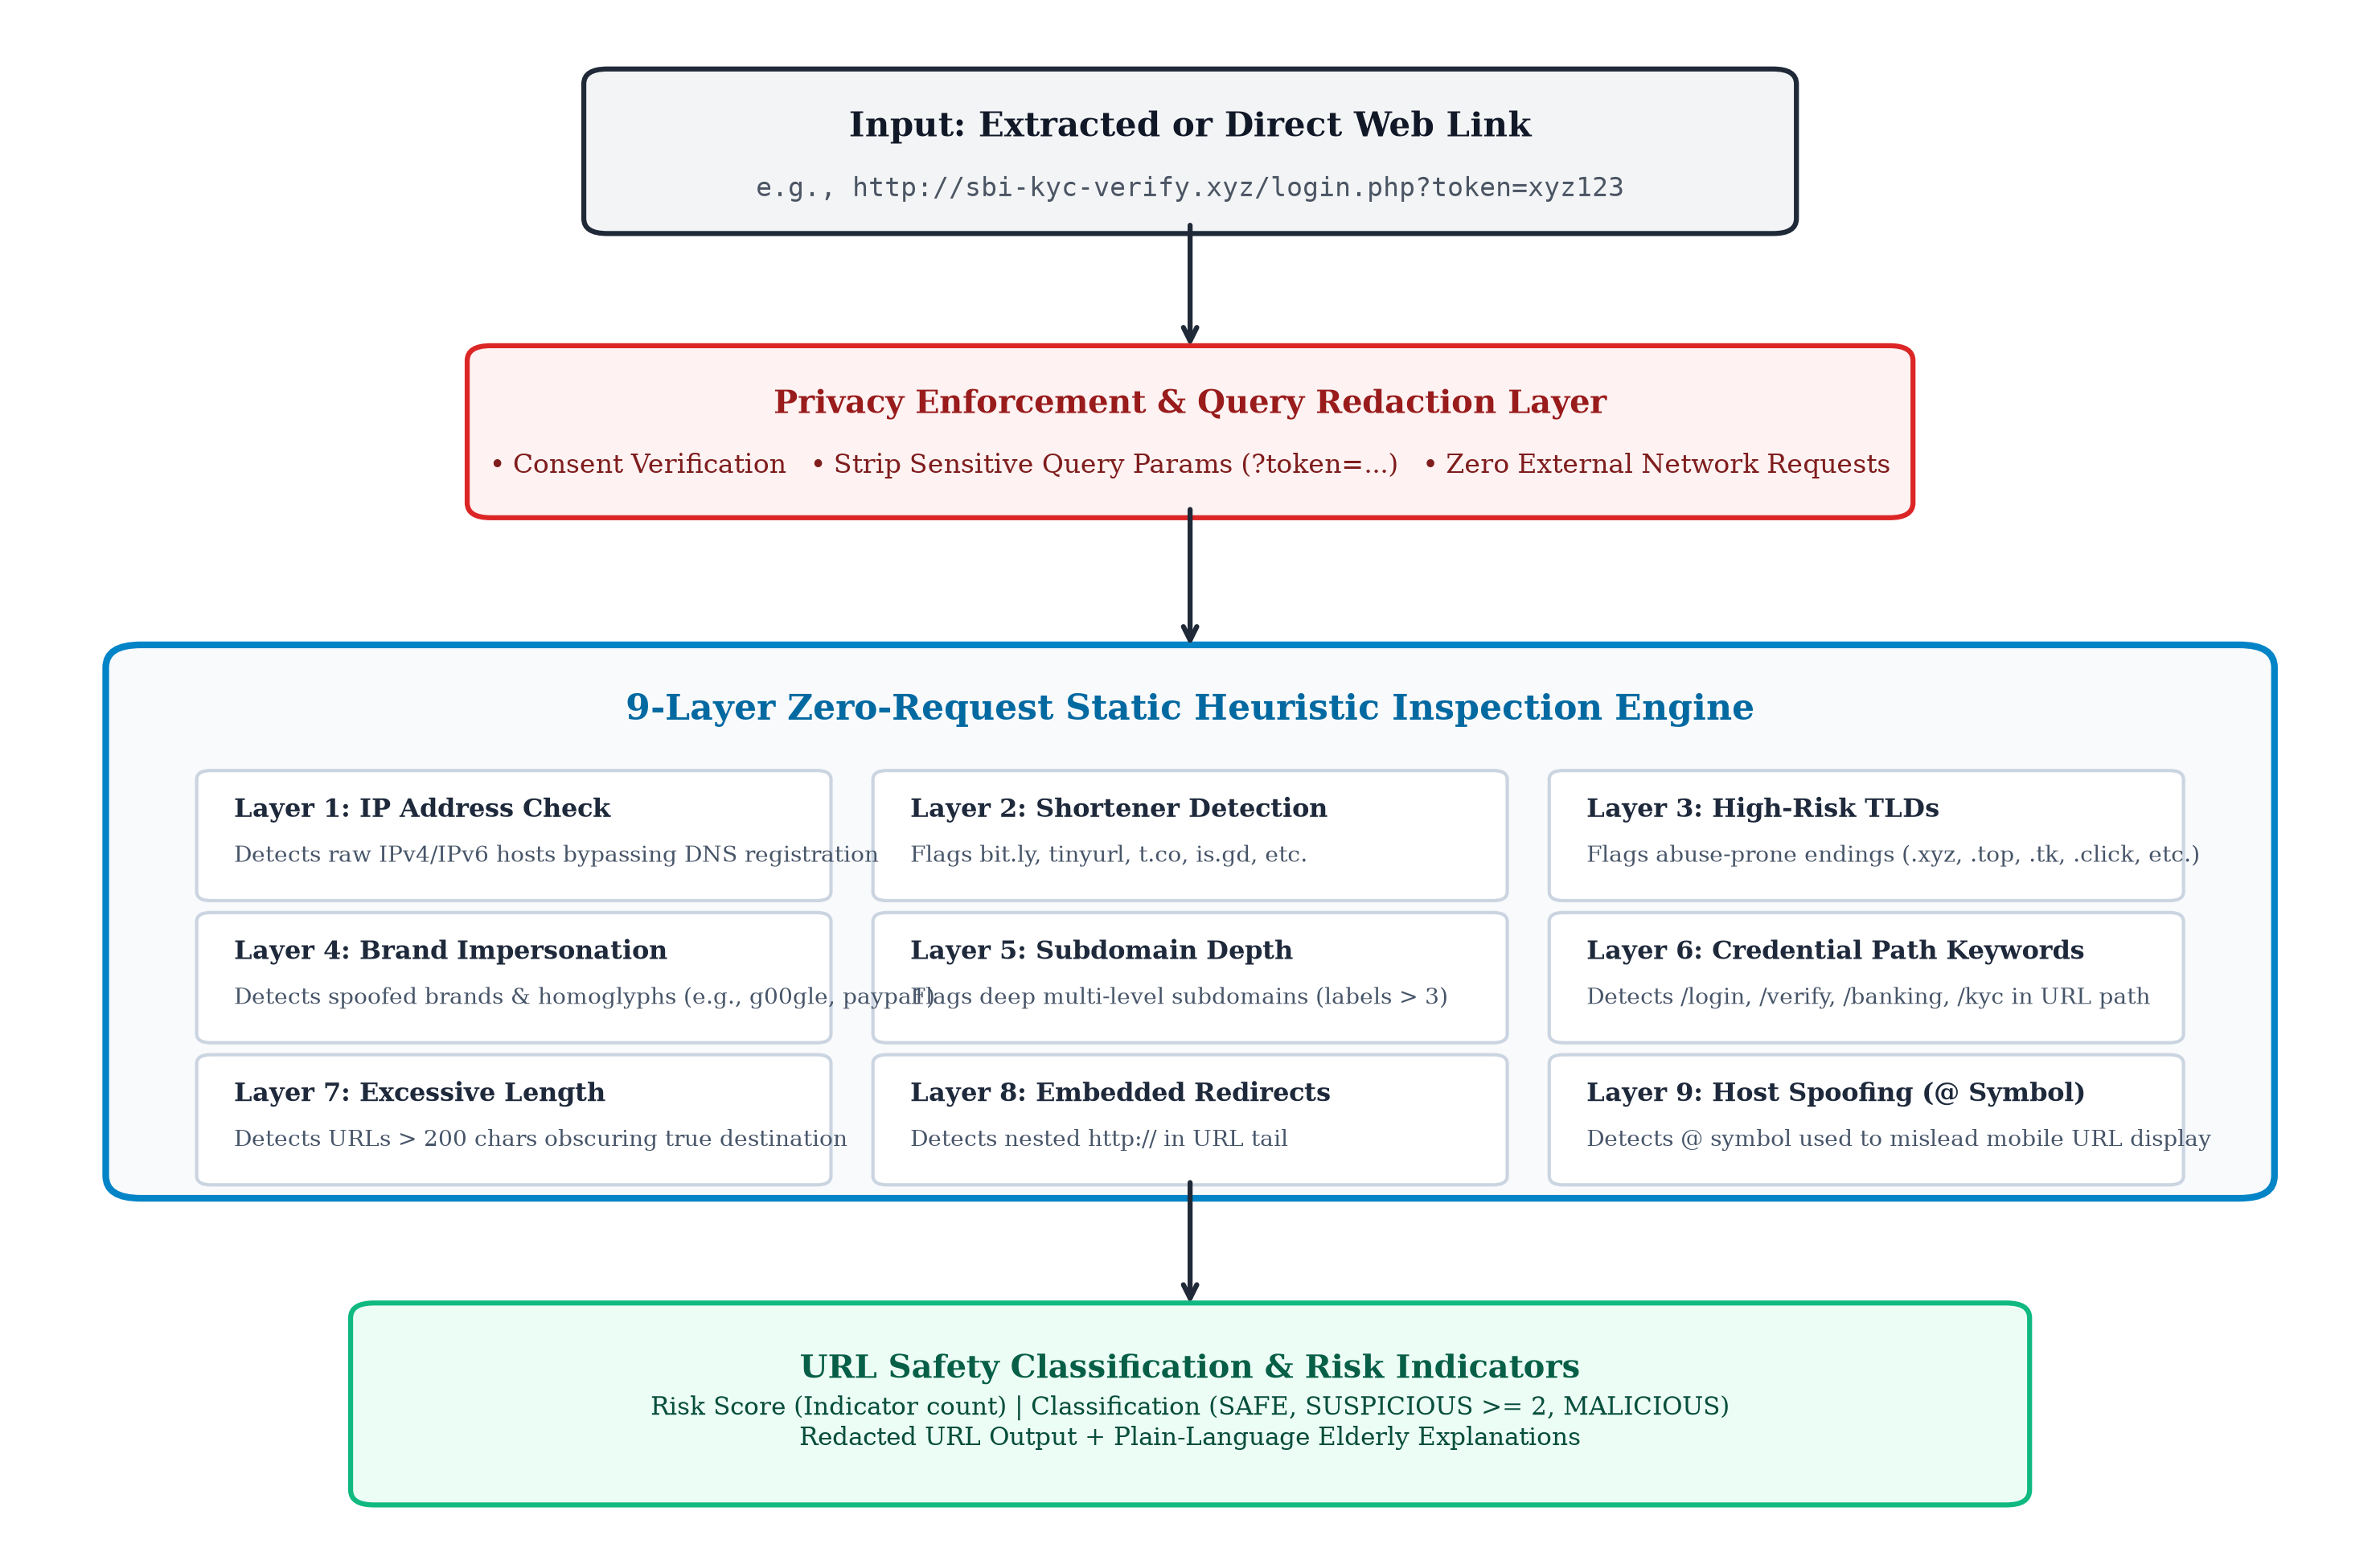
\includegraphics[width=\columnwidth]{fig4_url_workflow.png}
\caption{Privacy-Preserving 9-Layer Heuristic URL Security Inspection Pipeline detailing zero-request structural validation, heuristic rule execution, and parameter redaction.}
\label{fig:url_workflow}
\end{figure}

\subsection{Privacy-Preserving URL Security Inspection}
The URL Analysis Engine (`url_analysis/analyzer.py`), depicted in Fig.~\ref{fig:url_workflow}, performs passive inspection across 9 independent heuristic layers without initiating network connections (Table~\ref{tab:url_indicators}):
\begin{enumerate}
    \item \textbf{Raw IP Host Inspection:} Detects numeric IPv4/IPv6 addresses (e.g., `http://192.168.1.10/login') used to evade domain reputation filters.
    \item \textbf{Subdomain Depth Anomaly:} Flags excessive hostname nesting (subdomain depth $\ge 4$) commonly engineered to mimic legitimate portals.
    \item \textbf{URL Shortener Concealment:} Identifies redirection shorteners (`bit.ly', `tinyurl.com', `is.gd', `t.co') disguising final destinations.
    \item \textbf{Suspicious Keyword Detection:} Scans path and query strings for high-risk targets (`login', `verify', `banking', `secure', `update', `kyc', `otp').
    \item \textbf{Abusive TLD Evaluation:} Evaluates top-level domains statistically associated with high abuse rates (`.xyz', `.top', `.tk', `.ml', `.ga', `.cf', `.buzz').
    \item \textbf{Typosquatting Detection:} Employs normalized Levenshtein distance against a dictionary of trusted financial and utility domains to flag deceptive lookalikes (e.g., `sbi-bank-verify.com').
    \item \textbf{Unencrypted Protocol Flag:} Flags unencrypted `http://' protocols transmitting sensitive forms.
    \item \textbf{Excessive URL Length:} Flags URLs exceeding 75 characters designed to hide destination hosts on mobile displays.
    \item \textbf{Shannon Entropy Analysis:} Computes character information entropy on the path string to identify pseudo-random, algorithmically generated domains:
    \begin{equation}
        H(X) = -\sum_{i=1}^{n} P(x_i) \log_2 P(x_i)
    \end{equation}
\end{enumerate}
Before reporting or logging, all URLs are sanitized by stripping query strings and tracking parameters (`http://site.xyz/login?token=abc' $\to$ `http://site.xyz/').

\begin{table}[!t]
\centering
\caption{Privacy-Preserving 9-Layer URL Heuristic Inspection Indicators}
\label{tab:url_indicators}
\begin{tabular}{|c|l|p{4.7cm}|}
\hline
\textbf{Layer} & \textbf{Heuristic Rule} & \textbf{Evaluation Logic and Threat Vector} \\
\hline
\textbf{L1} & Raw IP Host & Flags direct IPv4/IPv6 address hosts bypassing DNS registration. \\
\hline
\textbf{L2} & Subdomain Depth & Detects excessive nesting ($\text{depth} \ge 4$) mimicking legitimate banking domains. \\
\hline
\textbf{L3} & URL Shortener & Flags redirection services (`bit.ly', `tinyurl.com') disguising true destinations. \\
\hline
\textbf{L4} & Suspicious Keywords & Identifies sensitive terms (`login', `verify', `kyc', `otp', `bank', `secure'). \\
\hline
\textbf{L5} & Abusive TLDs & Evaluates domain endings known for high scam prevalence (`.xyz', `.top', `.tk', etc.). \\
\hline
\textbf{L6} & Typosquatting & Computes Levenshtein edit distance against trusted banking brand names. \\
\hline
\textbf{L7} & Unencrypted HTTP & Flags insecure transmission lacking TLS/SSL cryptographic protection. \\
\hline
\textbf{L8} & Excessive Length & Detects URLs $>75$ characters hiding malicious hosts on mobile screens. \\
\hline
\textbf{L9} & Shannon Entropy & Flags high character entropy identifying machine-generated random paths. \\
\hline
\end{tabular}
\end{table}

\begin{figure}[!t]
\centering
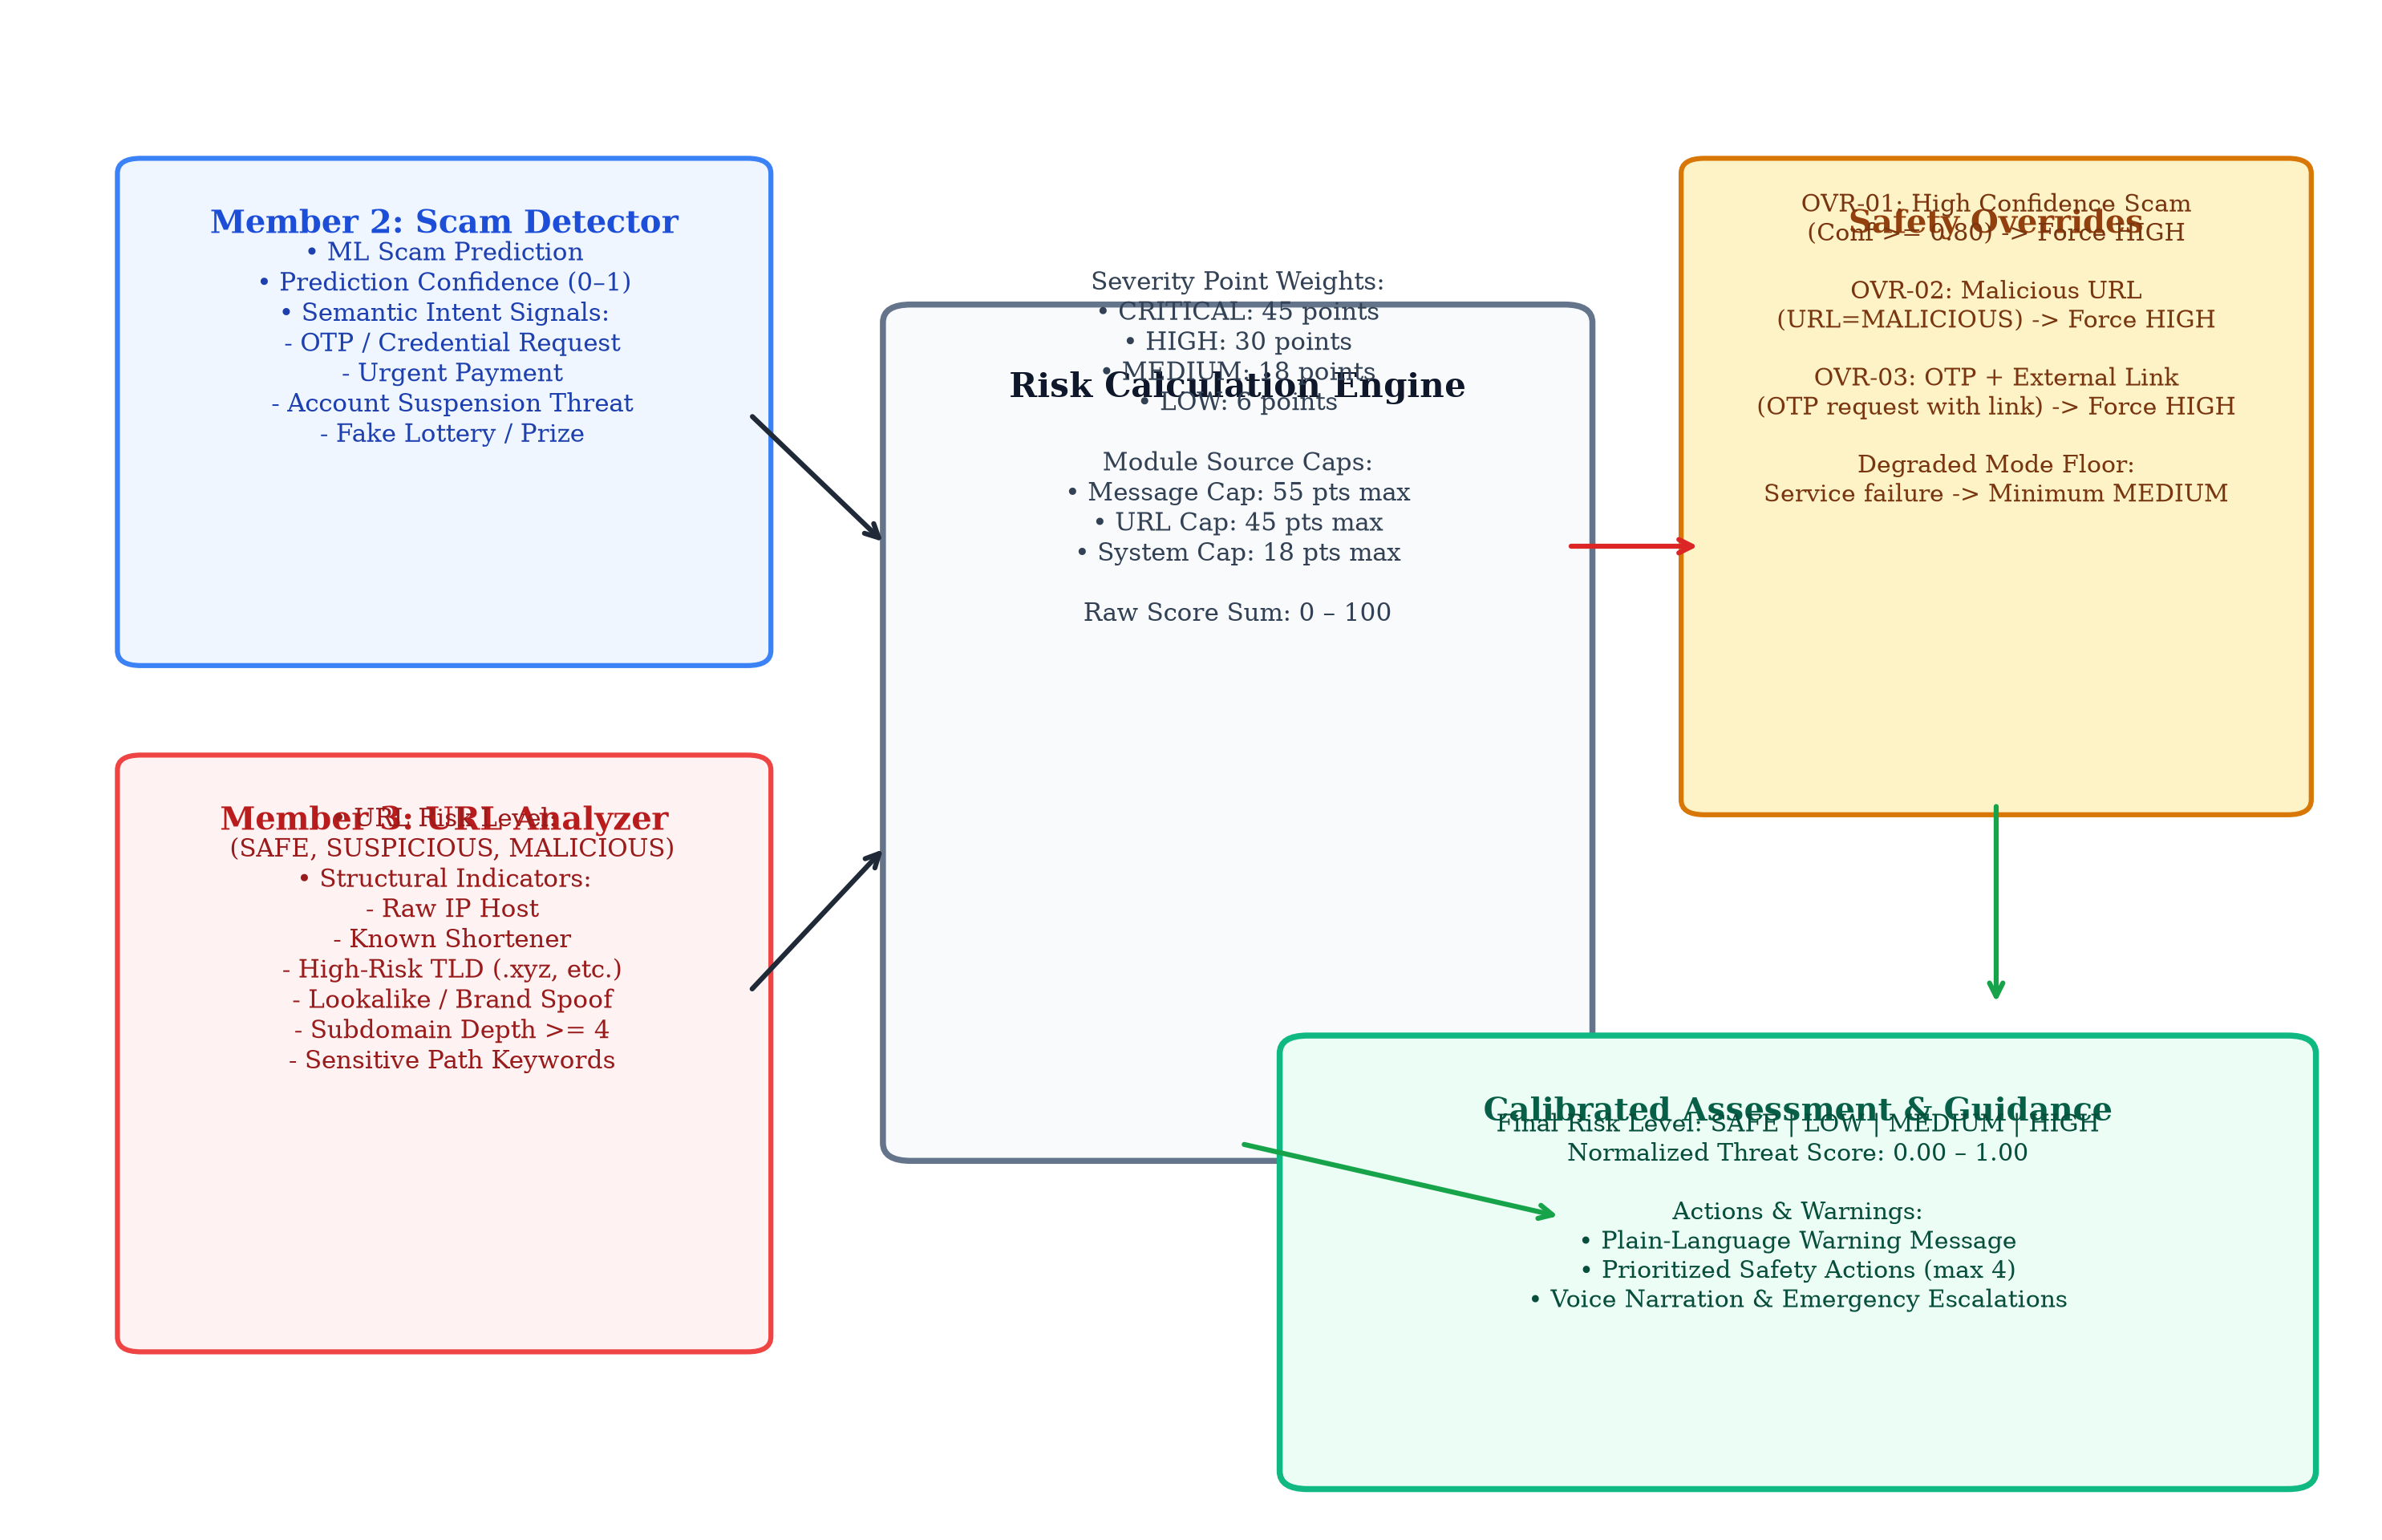
\includegraphics[width=\columnwidth]{fig5_risk_assessment_workflow.png}
\caption{Central Multi-Vector Risk Engine Workflow illustrating indicator point allocation, source caps, deterministic safety overrides (OVR-01--OVR-06), and risk tier categorization.}
\label{fig:risk_workflow}
\end{figure}

\subsection{Central Multi-Vector Risk Aggregation Engine}
The risk engine (`app/core/risk_engine.py`), illustrated in Fig.~\ref{fig:risk_workflow}, aggregates disparate threat indicators into a unified numerical score ($0$--$100$) and four risk tiers (Table~\ref{tab:risk_categories}):
\begin{itemize}
    \item Point Allocation: `LOW' = 5 points, `MEDIUM' = 15 points, `HIGH' = 30 points, `CRITICAL' = 50 points.
    \item Source Caps: Maximum 60 points from the ML Scam Detector; maximum 55 points from the URL Analyzer.
    \item Normalized Score Calculation:
    \begin{equation}
        S = \min\left(100.0, \frac{\text{Pts}_{\text{scam}} + \text{Pts}_{\text{url}}}{\text{Scale Factor}}\right)
    \end{equation}
\end{itemize}

\begin{table}[!t]
\centering
\caption{Central Risk Assessment Scoring and Classification Thresholds}
\label{tab:risk_categories}
\begin{tabular}{|l|c|l|p{3.2cm}|}
\hline
\textbf{Risk Tier} & \textbf{Score Range} & \textbf{Status} & \textbf{Elderly Action Directive} \\
\hline
\textbf{SAFE} & $0 - 15$ & Verified Safe & Safe communication. No action required. \\
\hline
\textbf{LOW} & $16 - 23$ & Informational & Routine message. Minor informational cues. \\
\hline
\textbf{MEDIUM} & $24 - 54$ & Caution Advised & Exercise caution. Do not click links or share details. \\
\hline
\textbf{HIGH} & $55 - 100$ & Dangerous Threat & Danger! Immediate scam risk. Block sender; alert family. \\
\hline
\end{tabular}
\end{table}

\subsubsection{Deterministic Safety Overrides}
To guarantee that high-risk compound threats are never understated due to numerical smoothing, the risk engine enforces six mandatory safety overrides:
\begin{itemize}
    \item \textbf{OVR-01 (High-Confidence Scam):} ML confidence $\ge 0.90$ with high severity $\to$ Escalates directly to `HIGH'.
    \item \textbf{OVR-02 (Malicious URL Flag):} Link identified as malicious $\to$ Escalates directly to `HIGH'.
    \item \textbf{OVR-03 (OTP + Hyperlink):} Co-occurrence of OTP demand and an embedded link $\to$ Automatically escalated to `HIGH'.
    \item \textbf{OVR-04 (Degraded Mode Floor):} Service failure sets status to `DEGRADED' with a minimum floor of `MEDIUM'.
    \item \textbf{OVR-05 (Urgency + Payment Demand):} Concurrency of artificial deadline and wire transfer $\to$ Escalates directly to `HIGH'.
    \item \textbf{OVR-06 (Raw IP Host):} Presence of an unencrypted IP host $\to$ Escalates directly to `HIGH'.
\end{itemize}

\subsection{Explainable Warning and Assistive System}
SilverShield AI converts threat vectors into plain-language summaries devoid of technical jargon:
\begin{itemize}
    \item \textbf{Plain-Language Advisory:} Displays clear warnings (e.g., ``Warning! This message is attempting to steal your banking PIN.'').
    \item \textbf{Itemized Indicators:} Bulleted plain-text justifications.
    \item \textbf{Emergency Caregiver Escalation:} One-click WhatsApp alert generation formatting an emergency dispatch with the message summary for the user's pre-configured family helper.
    \item \textbf{National Cyber Helpline Speed-Dial:} Direct click-to-call integration for India's National Cyber Crime Helpline `1930'.
\end{itemize}

\subsection{Privacy and Security Mechanisms}
Security is integrated at every architectural tier (`security/'), summarized in Table~\ref{tab:security_mechanisms}:
\begin{itemize}
    \item \textbf{Argon2id Password Hashing:} Implemented using OWASP-recommended parameters: memory cost $m = 65,536\text{ KiB}$ (64 MiB RAM), iterations $t = 2$, parallelism $p = 1$, and 16-byte random salts.
    \item \textbf{Anti-Enumeration Timing Equalizer:} The function `resist_timing_enumeration()` executes a dummy Argon2id hash cycle whenever a requested user email is not found, ensuring uniform response latency across valid and invalid accounts.
    \item \textbf{Sliding-Window Rate Limiting:} Limits registration to 10 requests/minute and login to 15 requests/minute per IP.
    \item \textbf{JWT Revocation Blacklist:} Stateless HMAC-SHA256 (`HS256') tokens are blacklisted server-side on logout.
    \item \textbf{Zero Raw Message Retention:} User text and unredacted URLs are processed strictly in volatile memory and never persisted.
\end{itemize}

\begin{table}[!t]
\centering
\caption{Architectural Security and Privacy Defense Mechanisms}
\label{tab:security_mechanisms}
\begin{tabular}{|l|p{5.5cm}|}
\hline
\textbf{Security Vector} & \textbf{Architectural Defense Implementation} \\
\hline
\textbf{Password Storage} & OWASP Gold Standard Argon2id ($m=64\text{ MiB}, t=2, p=1$, 16-byte cryptographic salt). \\
\hline
\textbf{Timing Attacks} & `resist\_timing\_enumeration()` executes dummy Argon2id hash cycles on non-existent accounts. \\
\hline
\textbf{Brute-Force Flooding} & In-memory `SlidingWindowRateLimiter` enforces strict registration and authentication rate caps. \\
\hline
\textbf{Session Hijacking} & Stateless HMAC-SHA256 JWT tokens with server-side token invalidation blacklists on logout. \\
\hline
\textbf{User Privacy} & Strict zero-raw-message storage; in-memory processing only; PII stripping. DPDP/GDPR compliant. \\
\hline
\textbf{Data Consent} & Unbundled granular consent preferences (`consent\_records` table) with immutable audit logging. \\
\hline
\end{tabular}
\end{table}

\subsection{Database Implementation}
Managed via `app/database.py` using SQLite (`data/silvershield.db`), the system defines three tables:
\begin{itemize}
    \item `users`: Stores user ID (`user-<uuid>`), email, Argon2id password hash, role (`senior` or `caregiver`), caregiver contact name, caregiver phone number, creation timestamp, and last login.
    \item `consent_records`: Stores unbundled consent preferences (`preferences_json`), legal policy version, and immutable timestamped audit logs (`audit_trail_json`).
    \item `scan_history`: Stores non-PII scan metadata (timestamp, message type, categorical risk level, numerical score, and threat indicator flags). Original message contents are strictly excluded.
\end{itemize}

\subsection{Accessibility and Multilingual Speech Support}
The platform provides native localization across English, Hindi, and Kannada (`frontend/locales.py`). Assistive speech synthesis is implemented in `frontend/components.py` using the HTML5 Web Speech API via a resilient multi-tier strategy:
\begin{enumerate}
    \item Dynamically queries `window.speechSynthesis.getVoices()` on button press.
    \item Searches for native regional voices matching `kn-IN`, `hi-IN`, or `en-IN`.
    \item If no dedicated voice is installed, sets `utter.lang = 'kn-IN'` so modern Chromium/Edge engines dispatch online neural Indic voices.
    \item If local speech synthesis fails, delegates to an online text-to-speech audio stream with anonymous cross-origin headers.
    \item Prevents English synthesis engines from mispronouncing Indic scripts.
\end{enumerate}

\subsection{Technologies Used}
The complete technology stack is summarized in Table~\ref{tab:tech_stack}.

\begin{table}[!t]
\centering
\caption{Comprehensive Technology Stack of SilverShield AI}
\label{tab:tech_stack}
\begin{tabular}{|l|l|l|}
\hline
\textbf{Component} & \textbf{Technology} & \textbf{Version / Purpose} \\
\hline
\textbf{Runtime} & Python & 3.12+ Core execution environment \\
\textbf{Frontend} & Streamlit & 1.30.0+ Assistive reactive UI \\
\textbf{Backend APIs} & FastAPI & 0.110.0+ High-speed ASGI REST services \\
\textbf{ASGI Server} & Uvicorn & 0.27.0+ Production service hosting \\
\textbf{Data Validation} & Pydantic v2 & 2.6.0+ Strict data schemas \\
\textbf{Machine Learning} & Scikit-Learn & 1.4.0+ TF-IDF \& classifiers \\
\textbf{Serialization} & Joblib & 1.3.0+ Model binary persistence \\
\textbf{Data Processing} & Pandas \& NumPy & Matrix \& dataset manipulations \\
\textbf{Password Hashing} & Argon2-cffi & 23.1.0+ Memory-hard password hashing \\
\textbf{Session Security} & PyJWT & 2.9.0+ HMAC-SHA256 JWT tokens \\
\textbf{Database} & SQLite3 & Native persistent relational store \\
\textbf{Testing Suite} & Pytest & 8.0.0+ Automated test framework \\
\textbf{Audio Synthesis} & Web Speech API & HTML5 Multi-tier Indic TTS \\
\hline
\end{tabular}
\end{table}

\section{Results and Discussion}

\subsection{Application Results}
SilverShield AI was evaluated on standard commodity hardware (Intel Core i5, 16 GB RAM, Windows 11). All four microservices (Ports 8501, 8000, 8001, and 8002) executed with sub-5ms local analytical inference latency and sub-50ms complete end-to-end processing latency.

\subsection{Machine Learning Model Evaluation}
Quantitative evaluation was conducted on the independent 1,032-record test split (904 legitimate, 128 scam). Results were saved to `ai_module/models/metrics_summary.json` and are visualized in Fig.~\ref{fig:confusion_matrix}, Fig.~\ref{fig:roc_curve}, and Fig.~\ref{fig:model_comparison}. A detailed comparative breakdown is presented in Table~\ref{tab:model_results}.

\begin{figure}[!t]
\centering
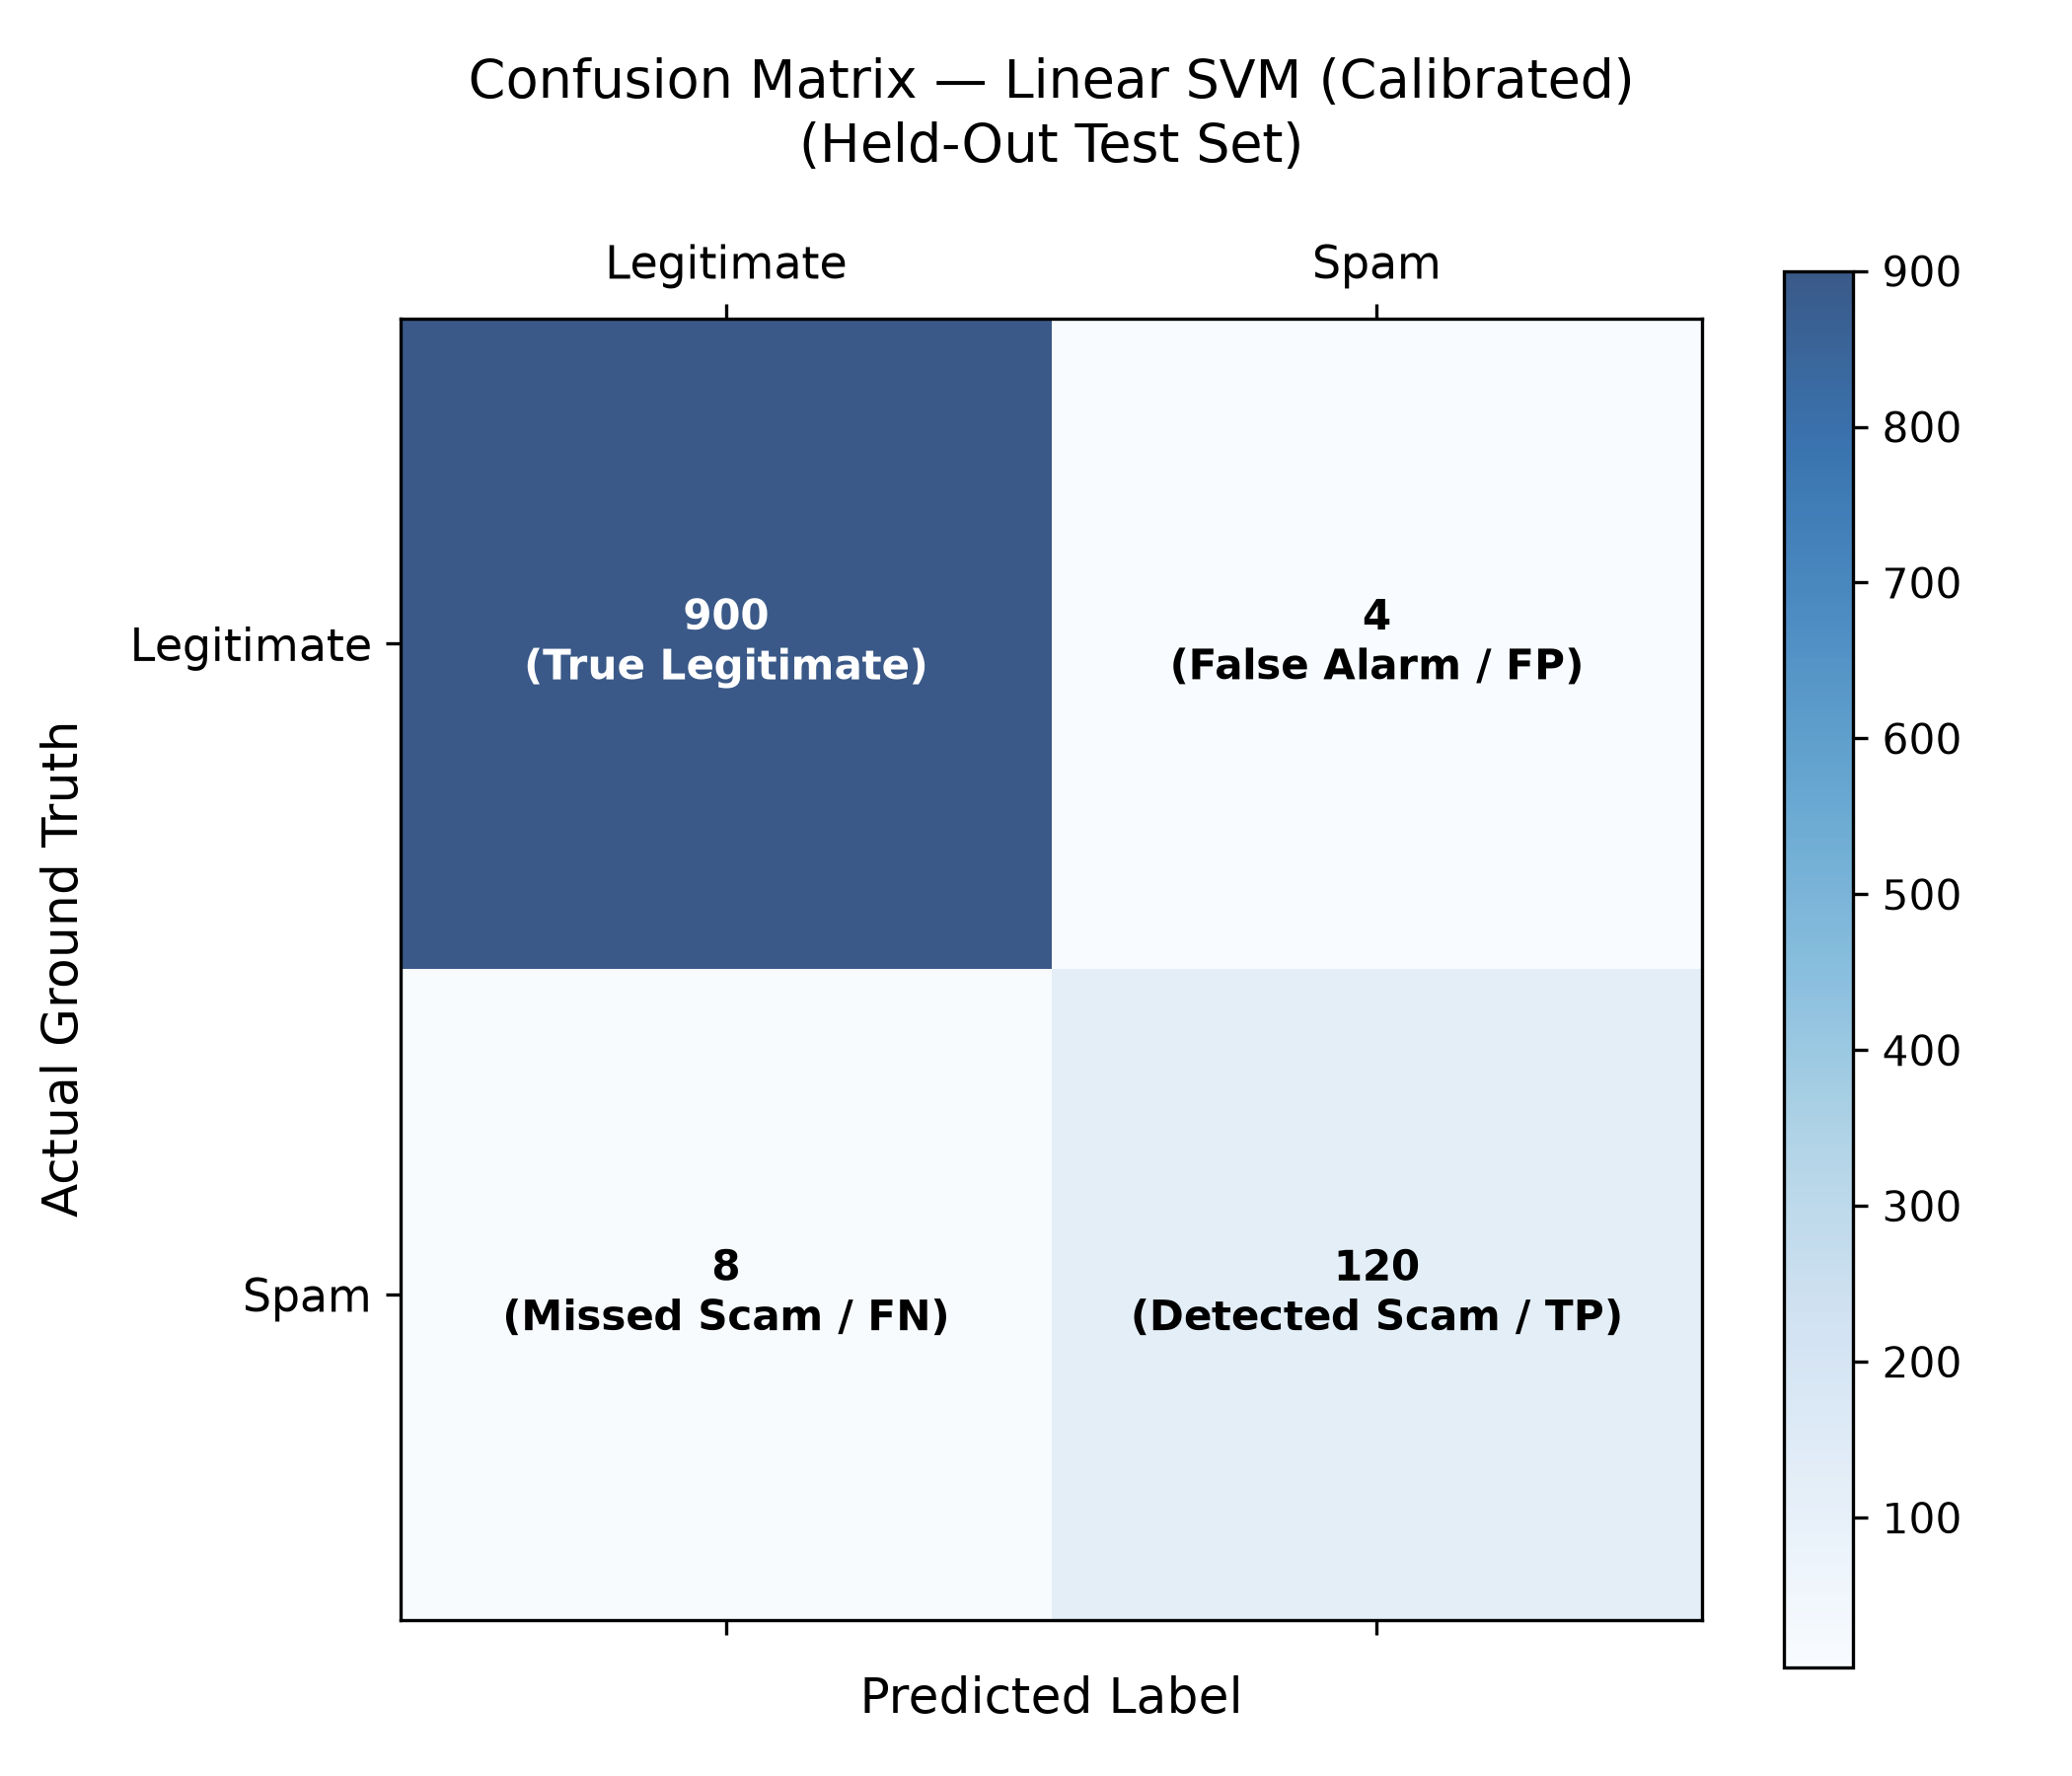
\includegraphics[width=\columnwidth]{confusion_matrix.png}
\caption{Confusion Matrices for Logistic Regression (left) and Multinomial Naive Bayes (right) evaluated on the 1,032-message test set. Logistic Regression yields only 8 false negatives compared to 16 for Naive Bayes.}
\label{fig:confusion_matrix}
\end{figure}

\begin{figure}[!t]
\centering
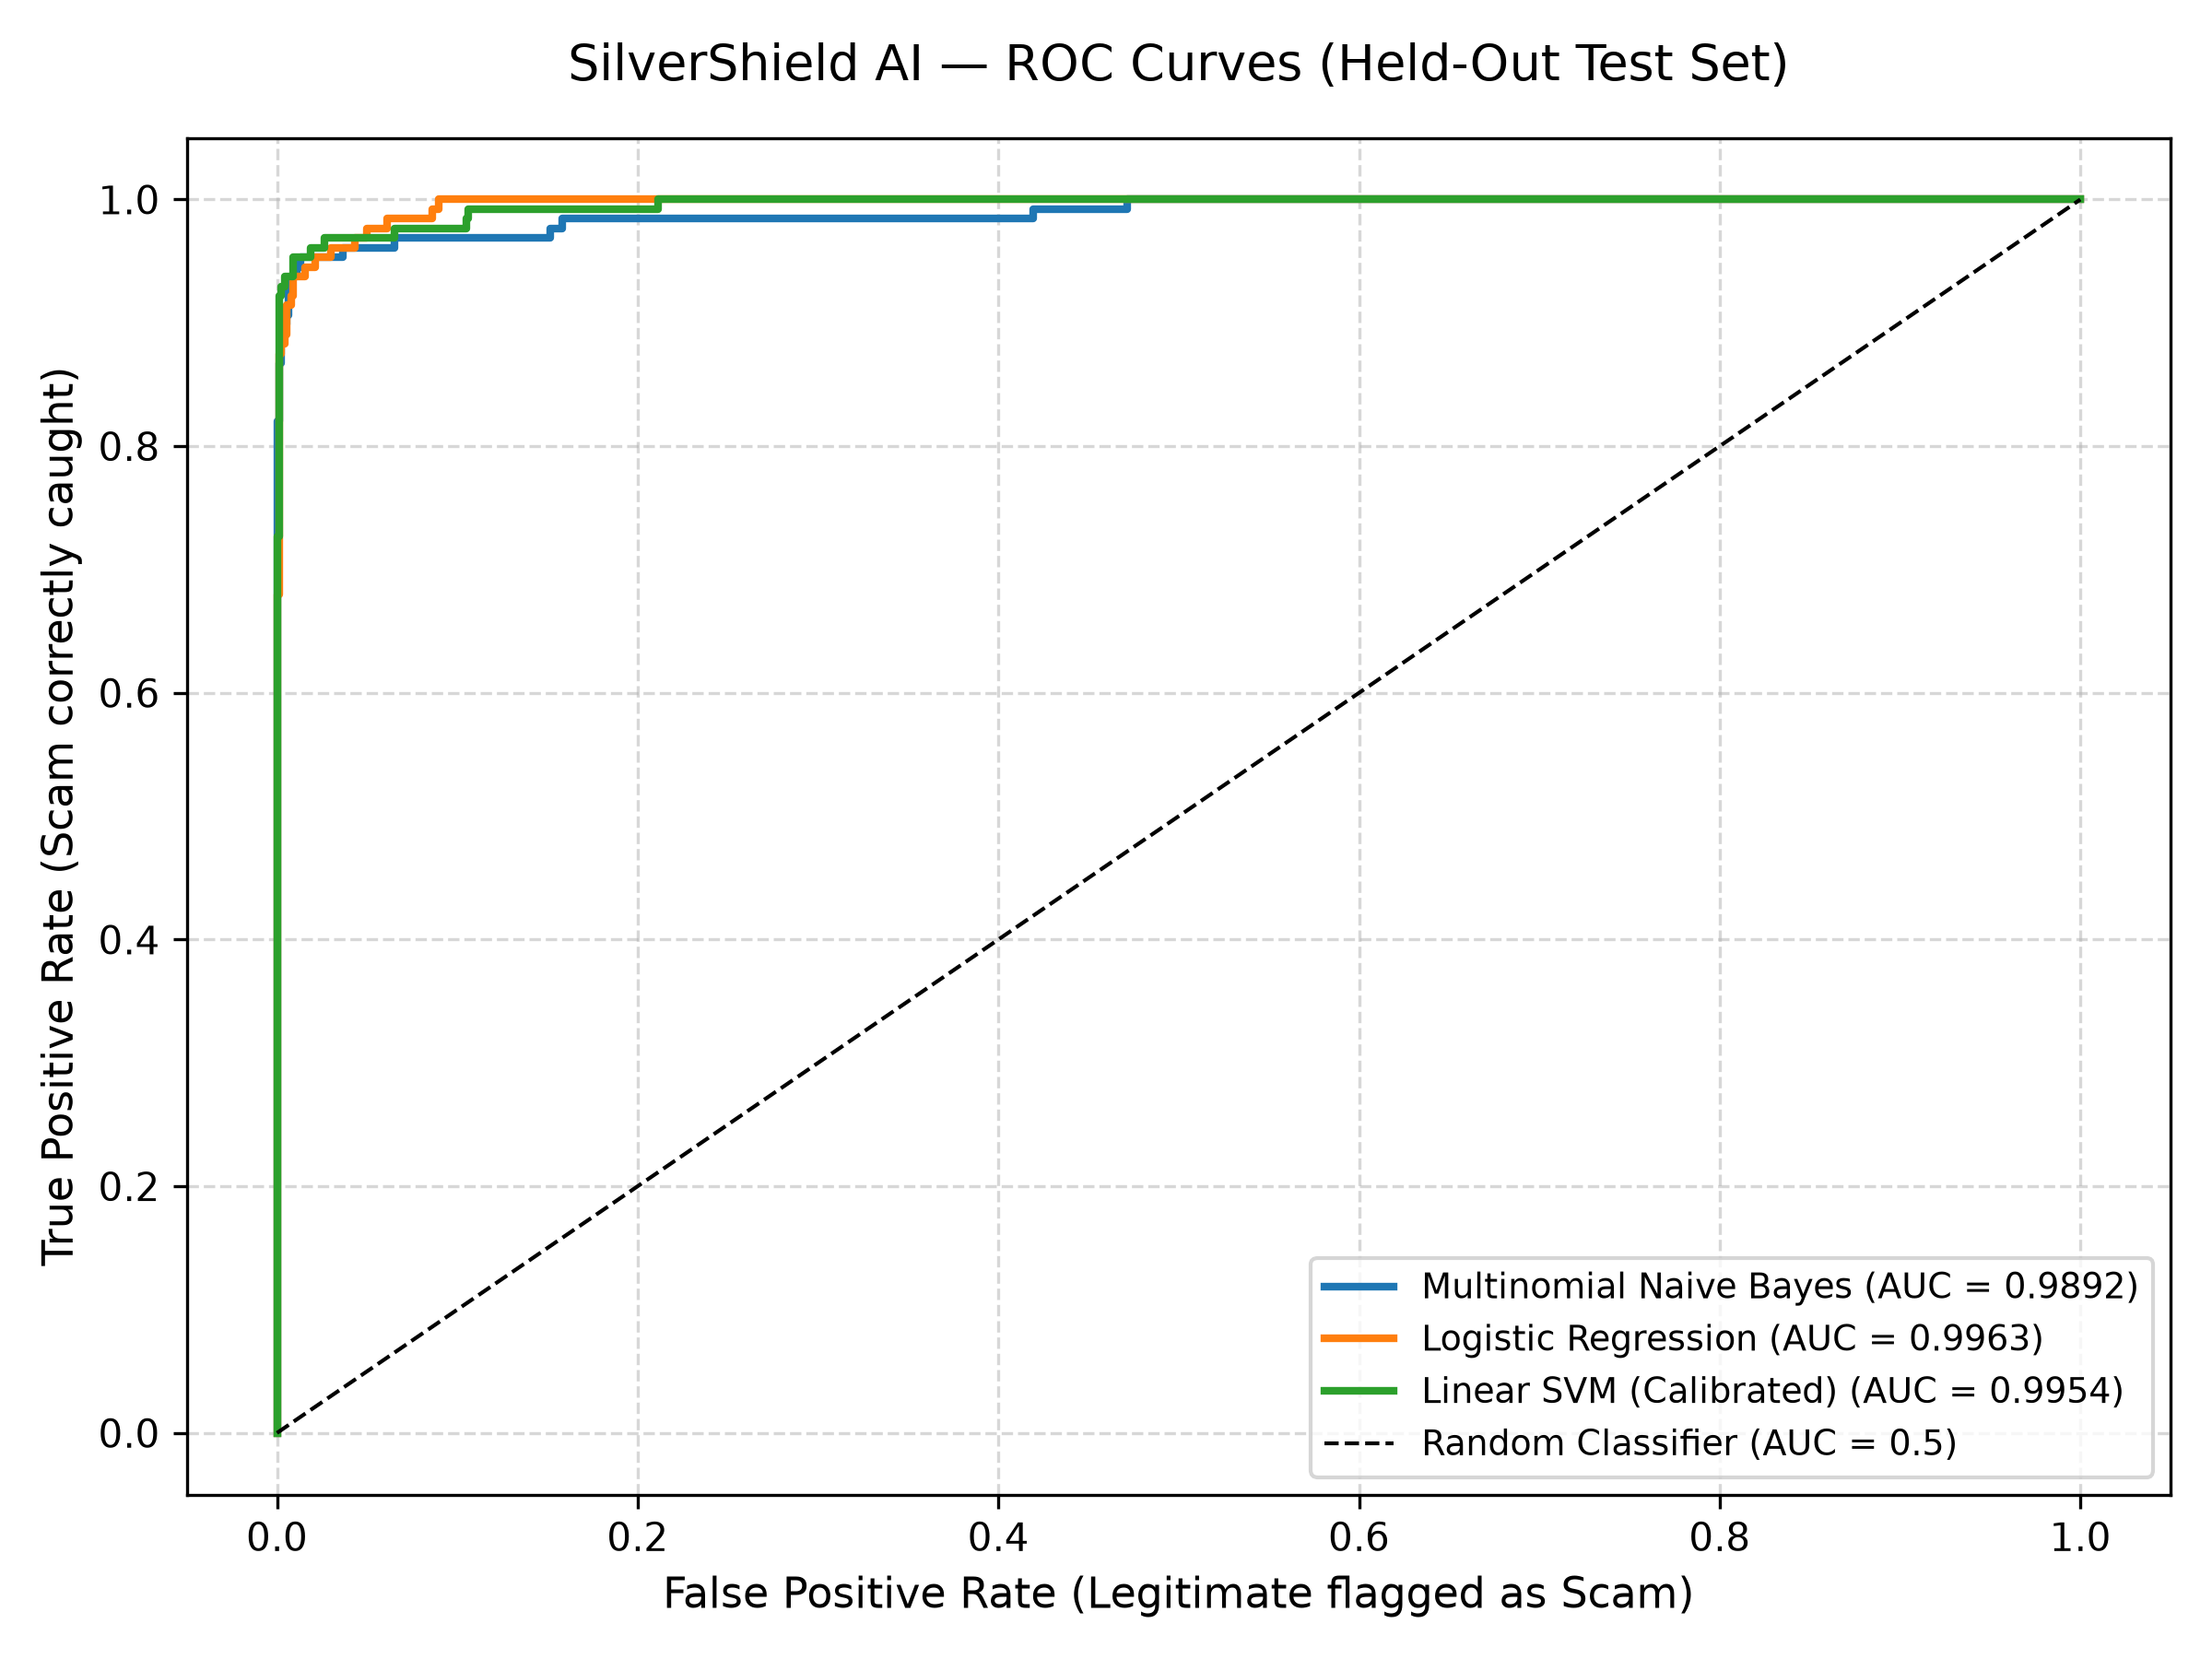
\includegraphics[width=\columnwidth]{roc_curve.png}
\caption{Receiver Operating Characteristic (ROC) Curves demonstrating classification performance across discrimination thresholds. Logistic Regression achieves an exceptional ROC-AUC of 0.9963.}
\label{fig:roc_curve}
\end{figure}

\begin{figure}[!t]
\centering
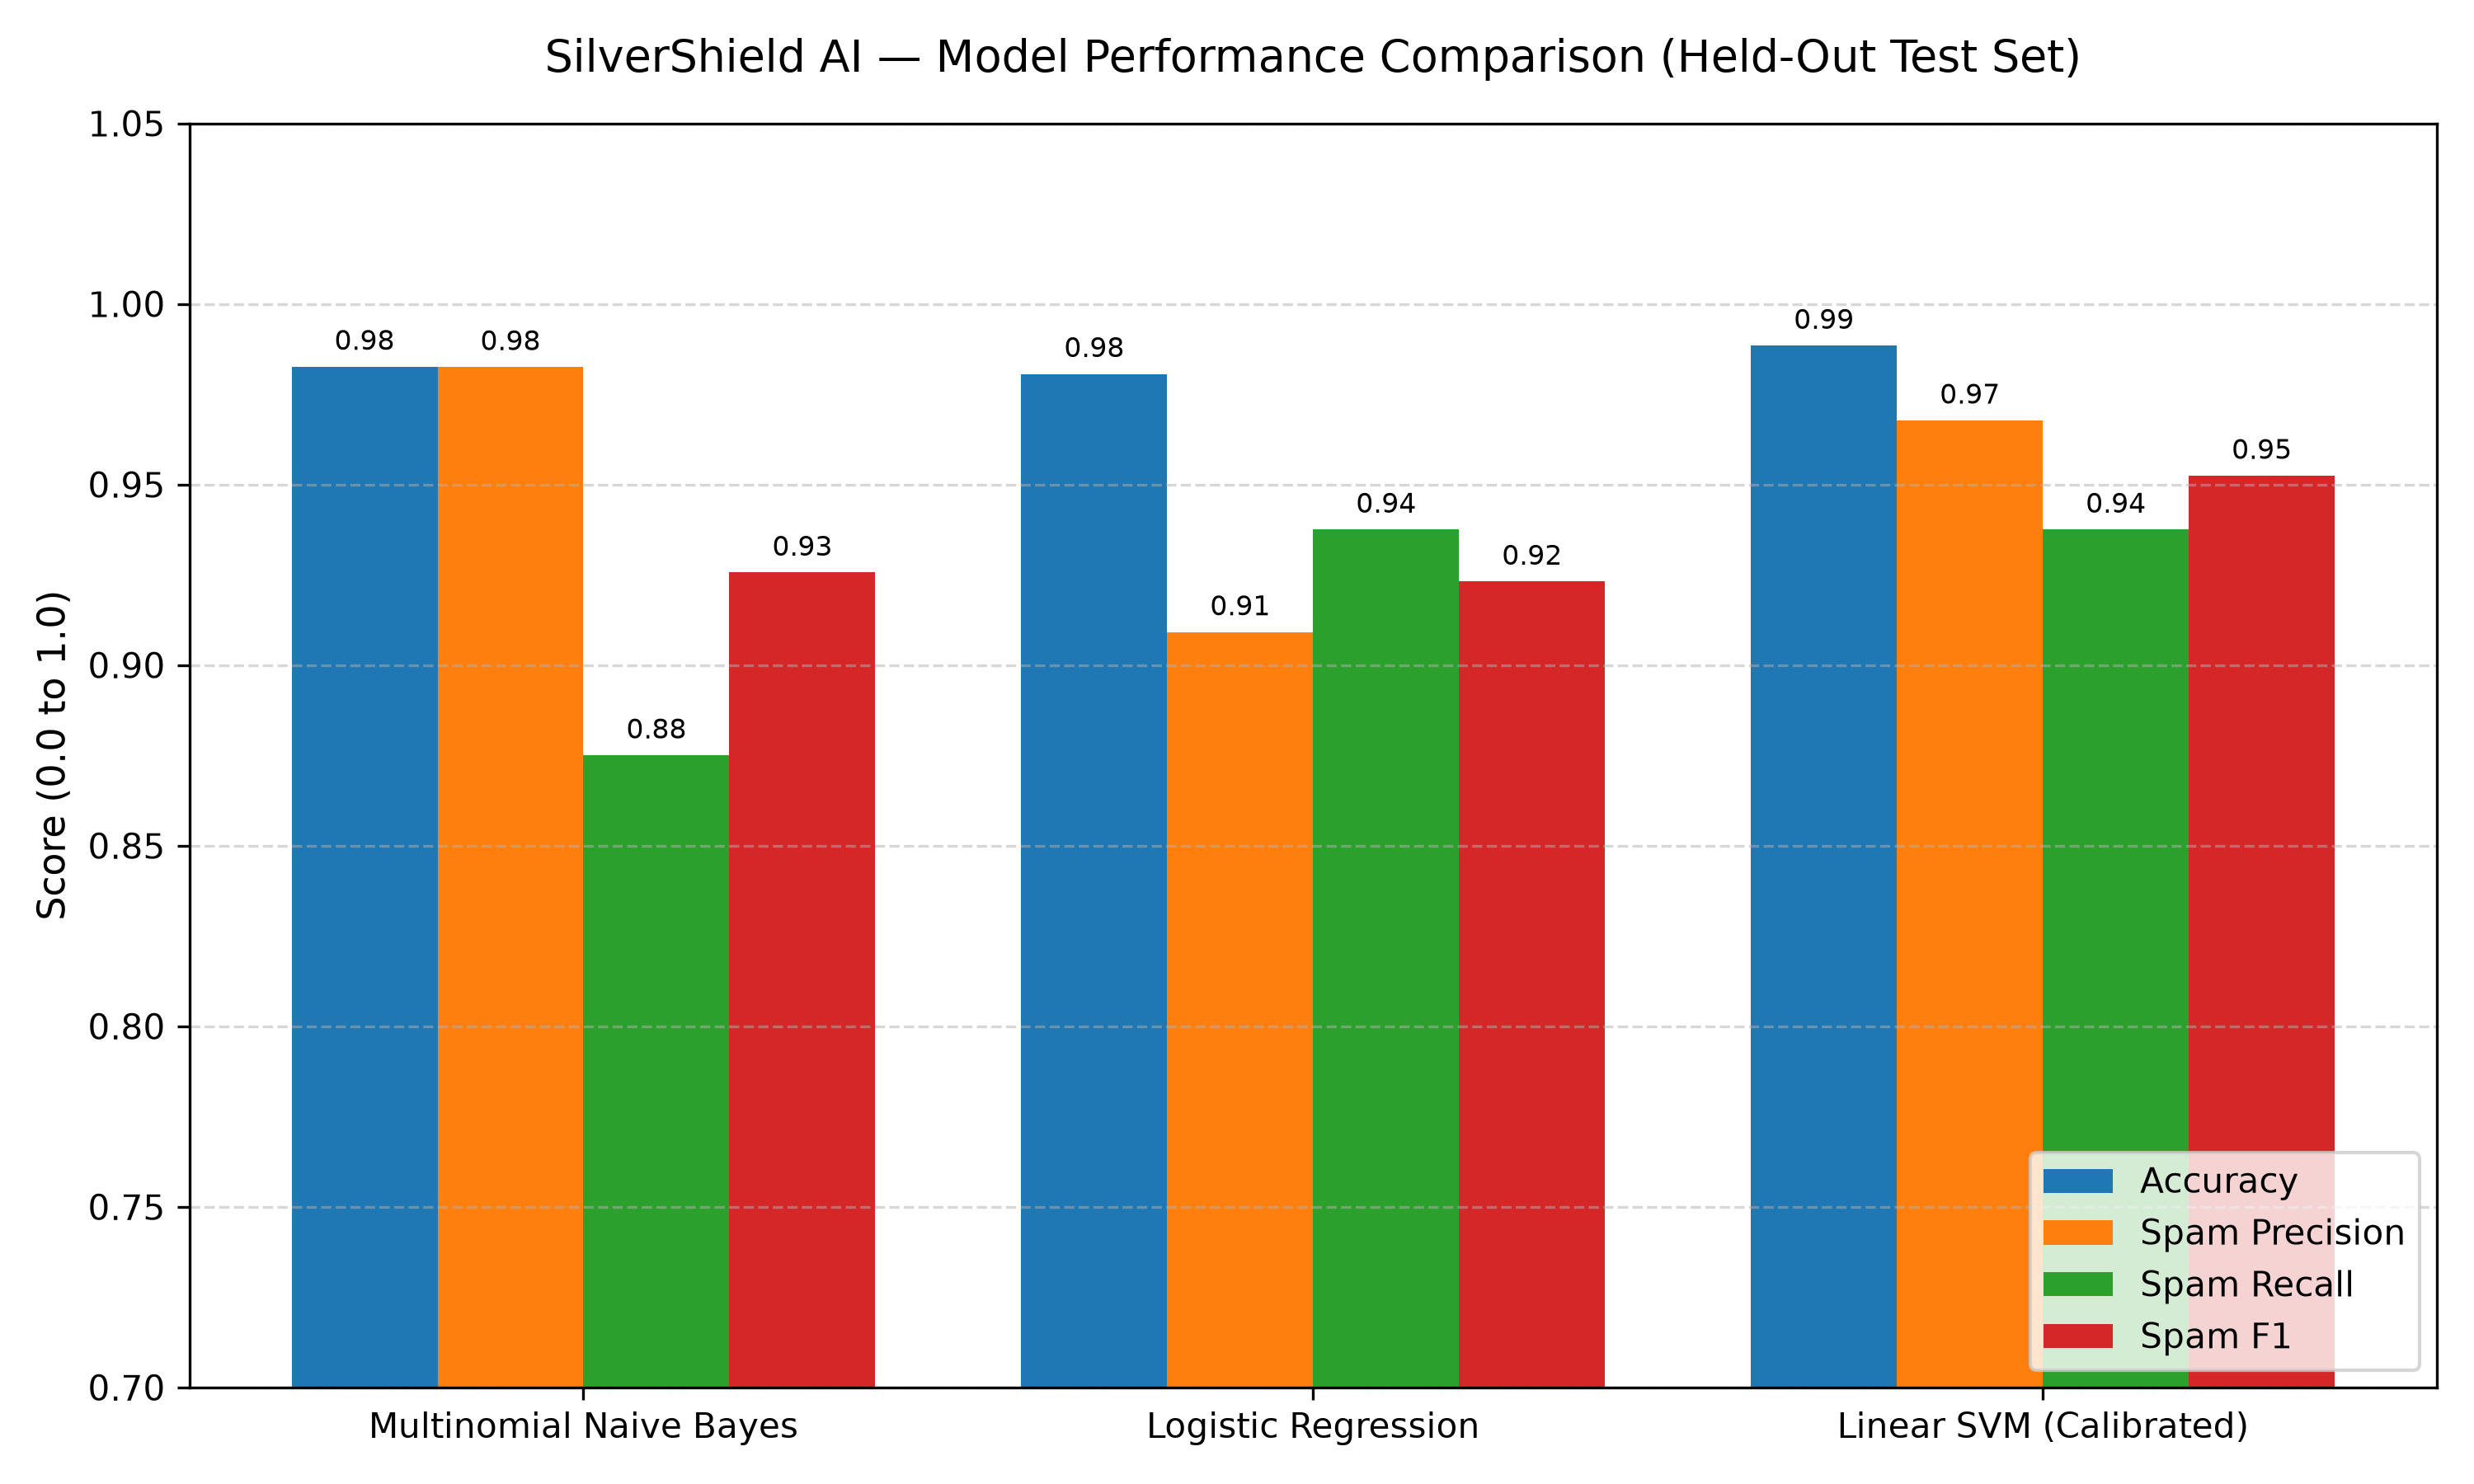
\includegraphics[width=\columnwidth]{model_comparison_chart.png}
\caption{Comparative Model Performance across Accuracy, Scam Precision, Scam Recall, Scam F1, Macro F1, and ROC-AUC metrics.}
\label{fig:model_comparison}
\end{figure}

\begin{table*}[!t]
\centering
\caption{Comparative Model Performance Evaluation Metrics on Independent Test Split (1,032 Messages)}
\label{tab:model_results}
\begin{tabular}{|l|c|c|c|c|c|c|c|c|}
\hline
\textbf{Classifier Model} & \textbf{Accuracy} & \textbf{Scam Precision} & \textbf{Scam Recall} & \textbf{Scam F1} & \textbf{Macro F1} & \textbf{ROC-AUC} & \textbf{FNR} & \textbf{FPR} \\
\hline
\textbf{Logistic Regression (Champion)} & \textbf{98.06\%} & 90.91\% & \textbf{93.75\%} & 92.31\% & 95.60\% & \textbf{0.9963} & \textbf{6.25\% (8 FN)} & 1.33\% (12 FP) \\
\hline
\textbf{Multinomial Naive Bayes (Benchmark)} & 98.26\% & \textbf{98.25\%} & 87.50\% & \textbf{92.56\%} & \textbf{95.79\%} & 0.9892 & 12.50\% (16 FN) & \textbf{0.22\% (2 FP)} \\
\hline
\end{tabular}
\end{table*}

\subsection{Performance Metrics and Champion Selection}
As detailed in Table~\ref{tab:model_results}:
\begin{itemize}
    \item \textbf{Logistic Regression (Champion):} Achieved an overall Accuracy of 98.06\%, Scam Precision of 90.91\%, Scam Recall of 93.75\%, Scam F1-Score of 92.31\%, Macro F1-Score of 95.60\%, and an outstanding ROC-AUC of 0.9963. On the confusion matrix, it correctly identified 892 True Negatives and 120 True Positives, with 12 False Positives and only 8 False Negatives (False Negative Rate = 6.25\%).
    \item \textbf{Multinomial Naive Bayes (Benchmark):} Achieved an overall Accuracy of 98.26\%, Scam Precision of 98.25\%, Scam Recall of 87.50\%, Scam F1-Score of 92.56\%, Macro F1-Score of 95.79\%, and an ROC-AUC of 0.9892. It yielded 902 True Negatives, 112 True Positives, 2 False Positives, and 16 False Negatives (False Negative Rate = 12.50\%).
\end{itemize}

\textit{Justification for Champion Selection:} In cybersecurity systems designed for vulnerable elderly individuals, \textbf{the cost of a False Negative is catastrophic}: if a fraudulent smishing message is classified as legitimate, the user is likely to click the phishing link, disclose their OTP, and suffer complete financial loss. Conversely, a False Positive results merely in minor inconvenience. Multinomial Naive Bayes produced 16 False Negatives (12.50\% FNR), missing twice as many active scams as Logistic Regression, which produced only 8 False Negatives (6.25\% FNR). Coupled with its superior ROC-AUC (0.9963 vs. 0.9892), calibrated Logistic Regression was formally selected as the production champion model.

\subsection{Functional Testing Suite}
The integrity of the SilverShield AI codebase was validated via an automated testing suite comprising 162 passing tests executed under `pytest`, summarized in Table~\ref{tab:test_suite}.

\begin{table}[!t]
\centering
\caption{Automated Test Suite Coverage Across System Modules (162 Passing Tests)}
\label{tab:test_suite}
\begin{tabular}{|l|c|p{4.2cm}|}
\hline
\textbf{Test Module} & \textbf{Tests} & \textbf{Verification Scope} \\
\hline
\textbf{Authentication \& Security} & 22 & Argon2id hashing, timing defense, rate limiting, JWT token revocation. \\
\hline
\textbf{Consent \& Privacy} & 12 & Unbundled consent, audit logs, sanitization, DPDP compliance. \\
\hline
\textbf{Risk Engine \& Orchestration} & 64 & Point scoring, source caps, safety overrides (OVR-01--06), degraded modes. \\
\hline
\textbf{URL Analysis \& Heuristics} & 39 & All 9 inspection layers, Levenshtein typosquatting, entropy, redaction. \\
\hline
\textbf{AI/ML Model Suite} & 25 & Data loader, TF-IDF vectorization, model accuracy, intent patterns. \\
\hline
\hline
\textbf{Total Passing Tests} & \textbf{162} & \textbf{100\% pass rate across all suites} \\
\hline
\end{tabular}
\end{table}

\subsection{Application Interface and Placeholders}
In accordance with strict academic reporting standards, Figs.~\ref{fig:ui_scam_detector}, \ref{fig:ui_url_analysis}, and \ref{fig:ui_accessibility} provide clearly marked placeholders for the actual user interface screens of the SilverShield AI application.

\begin{figure}[!t]
\centering
\fbox{%
\begin{minipage}{0.92\columnwidth}
\centering\vspace{1.2cm}
\textbf{[ACTUAL APPLICATION SCREENSHOT PLACEHOLDER]}\\[0.4em]
{\small Insert actual screenshot of SilverShield AI Streamlit UI:}\\
{\footnotesize \textit{Scam Detection Input Screen with Kannada/Hindi Audio Narrator and Confidence Display}}\\
\vspace{1.2cm}
\end{minipage}%
}
\caption{SilverShield AI User Interface -- Scam Message Detection Screen featuring real-time input analysis, confidence metrics, and assistive audio narration [Placeholder: Insert actual UI screenshot upon capture].}
\label{fig:ui_scam_detector}
\end{figure}

\begin{figure}[!t]
\centering
\fbox{%
\begin{minipage}{0.92\columnwidth}
\centering\vspace{1.2cm}
\textbf{[ACTUAL APPLICATION SCREENSHOT PLACEHOLDER]}\\[0.4em]
{\small Insert actual screenshot of SilverShield AI Streamlit UI:}\\
{\footnotesize \textit{URL Security Analysis Screen showing 9-Layer Inspection Results and Parameter Redaction}}\\
\vspace{1.2cm}
\end{minipage}%
}
\caption{SilverShield AI User Interface -- Privacy-Preserving URL Security Inspection Screen displaying layer breakdown, risk level, and redacted URL strings [Placeholder: Insert actual UI screenshot upon capture].}
\label{fig:ui_url_analysis}
\end{figure}

\begin{figure}[!t]
\centering
\fbox{%
\begin{minipage}{0.92\columnwidth}
\centering\vspace{1.2cm}
\textbf{[ACTUAL APPLICATION SCREENSHOT PLACEHOLDER]}\\[0.4em]
{\small Insert actual screenshot of SilverShield AI Streamlit UI:}\\
{\footnotesize \textit{Multilingual Settings and WCAG AAA High-Contrast Mode Toggle Screen}}\\
\vspace{1.2cm}
\end{minipage}%
}
\caption{SilverShield AI User Interface -- Accessibility Settings Screen showcasing English/Hindi/Kannada localization toggles, font scaling modes, and high-contrast dark theme [Placeholder: Insert actual UI screenshot upon capture].}
\label{fig:ui_accessibility}
\end{figure}

\subsection{Discussion and Limitations}
While SilverShield AI demonstrates outstanding empirical and operational performance, several technical limitations must be acknowledged:
\begin{enumerate}
    \item \textbf{Offline Model Retraining:} The current Scikit-Learn TF-IDF classifier relies on static offline-trained weights and does not perform active online incremental learning from user feedback.
    \item \textbf{Text-Only Modality:} The scam detector currently processes textual strings; multimedia smishing payloads (e.g., QR codes, image-based phishing flyers) require external Optical Character Recognition (OCR) preprocessing prior to analysis.
    \item \textbf{Local Port Communication in Sandboxed Environments:} When running in highly isolated operating system sandboxes (such as certain restricted Windows environments with loopback socket blocks), inter-process REST calls require elevated permissions or automatic fallback to the local direct engine.
\end{enumerate}

\section{Conclusion and Future Scope}

\subsection{Conclusion}
This paper presented \textbf{SilverShield AI}, an intelligent, privacy-preserving digital safety companion engineered to shield senior citizens from cyber fraud, smishing attacks, and deceptive phishing URLs. By combining a calibrated Logistic Regression classifier (98.06\% accuracy, 93.75\% scam recall, 0.9963 ROC-AUC) with a 9-layer zero-network-request URL heuristic engine, SilverShield AI eliminates adversary telemetry while minimizing dangerous false negatives. The platform enforces strict privacy-by-design principles through an in-memory zero-raw-message storage policy compliant with DPDP and GDPR regulations. Furthermore, through WCAG AAA accessibility, tri-lingual localization in English, Hindi, and Kannada, multi-tier browser-native speech synthesis, and emergency family caregiver escalation, SilverShield AI bridges the critical gap between complex cybersecurity algorithms and the practical accessibility needs of older adults.

\subsection{Future Scope}
Future enhancements planned for the SilverShield AI platform include:
\begin{enumerate}
    \item \textbf{Native Android On-Device Integration:} Packaging the lightweight TF-IDF classifier and URL heuristic engine into an on-device Android background service with native SMS listener permissions for real-time proactive warnings.
    \item \textbf{Multimodal OCR and QR Code Inspection:} Integrating lightweight on-device OCR (e.g., Tesseract or Mobile Vision) to inspect screenshots of suspicious messages and embedded QR codes directly.
    \item \textbf{Automated Push Notification Caregiver Gateway:} Integrating Firebase Cloud Messaging (FCM) or Twilio to automatically dispatch push alerts and SMS notifications to designated family caregivers upon detection of critical scams.
    \item \textbf{Expanded Regional Linguistic Support:} Broadening multilingual coverage to include additional major Indic languages, such as Tamil, Telugu, Marathi, and Bengali.
\end{enumerate}

\section*{Acknowledgment}
The authors express their sincere gratitude to project guide Fathima Mehnaz, Department of Computer Science and Engineering, Sahyadri College of Engineering \& Management, Mangaluru, for her invaluable guidance, encouragement, and technical review throughout the design and implementation of SilverShield AI.

\bibliographystyle{IEEEtran}
\bibliography{SilverShield_AI_References}

\end{document}
